\documentclass{whiteboard}
\begin{document}
\begin{frame}[plain,t]
\bbcover{Combinadores}{Base $SK$}{Prof. Edson Alves}{Campus UnB Gama: Faculdade de Ciências e Tecnologias em Engenharia}

\end{frame}
\begin{frame}[plain,t]
\begin{tikzpicture}
\node[draw,opacity=0] at (0, 0) {x};
\node[draw,opacity=0] at (14, 8) {x};

	\node[anchor=west] (title) at (0.0, 7.0) { \Large \bbbold{Base SK} };

\end{tikzpicture}
\end{frame}
\begin{frame}[plain,t]
\begin{tikzpicture}
\node[draw,opacity=0] at (0, 0) {x};
\node[draw,opacity=0] at (14, 8) {x};

	\node[anchor=west] (title) at (0.0, 7.0) { \Large \bbbold{Base SK} };


	\node[] (a) at (4.0, 3.5) { 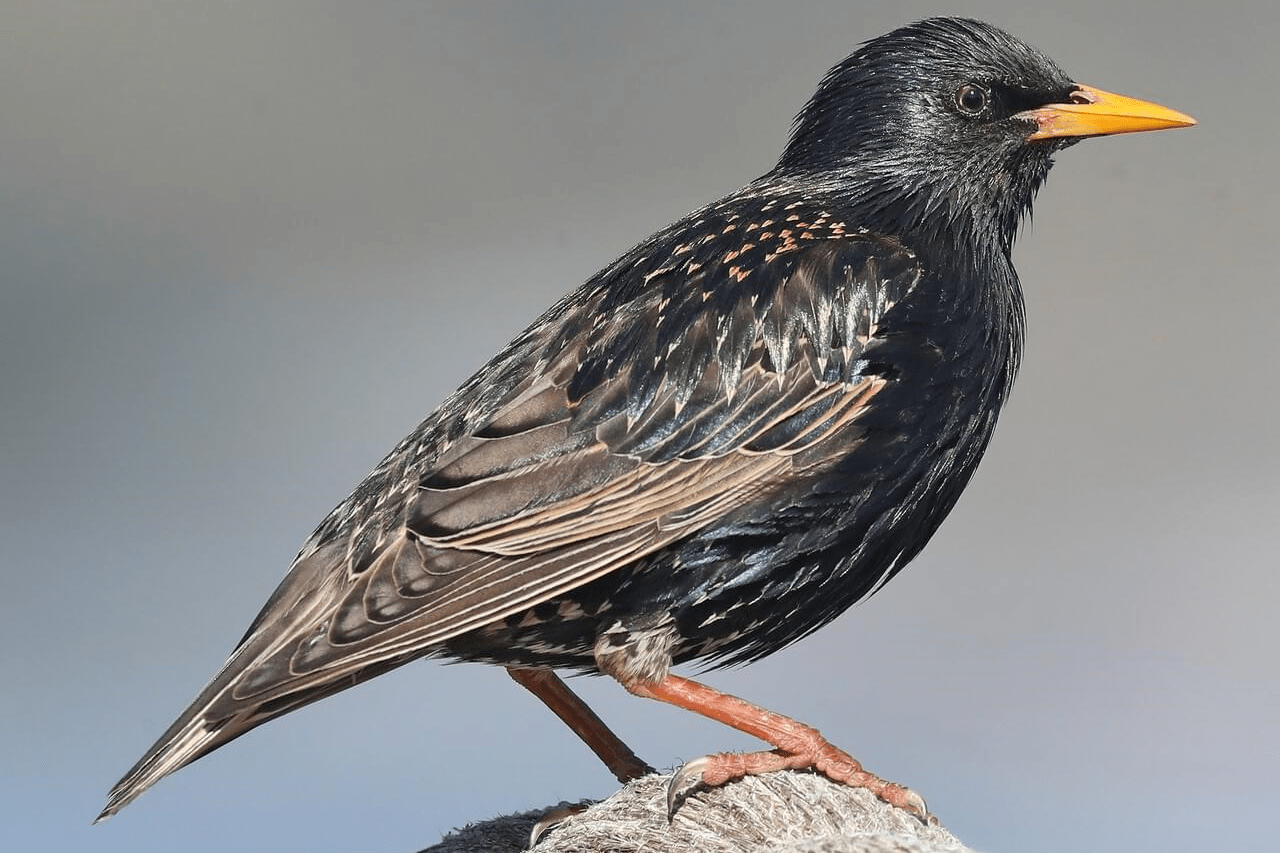
\includegraphics[scale=0.2]{figs/starling.png} };

	\node[] (a1) at (4.0, 0.75) { \bbtext{Estorninho (\bbenglish{starling})} };

\end{tikzpicture}
\end{frame}
\begin{frame}[plain,t]
\begin{tikzpicture}
\node[draw,opacity=0] at (0, 0) {x};
\node[draw,opacity=0] at (14, 8) {x};

	\node[anchor=west] (title) at (0.0, 7.0) { \Large \bbbold{Base SK} };


	\node[] (a) at (4.0, 3.5) { 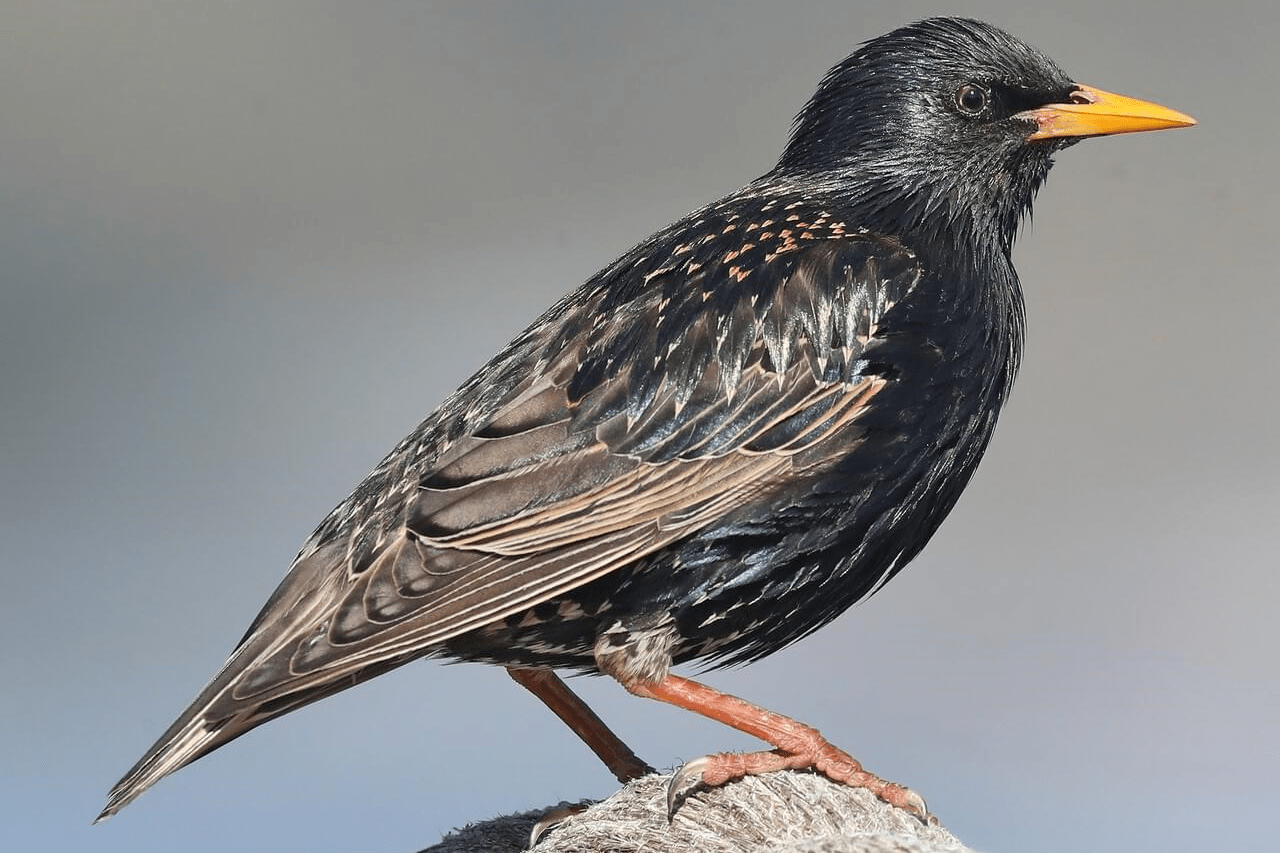
\includegraphics[scale=0.2]{figs/starling.png} };

	\node[] (a1) at (4.0, 0.75) { \bbtext{Estorninho (\bbenglish{starling})} };


	\node[] (b) at (11.0, 3.5) { 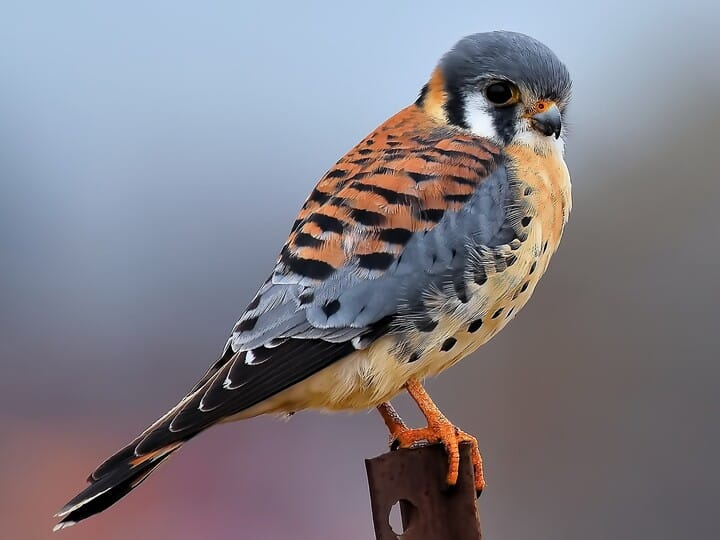
\includegraphics[scale=0.235]{figs/kestrel.jpg} };

	\node[] (b1) at (11.0, 0.75) { \bbtext{Cernícalo americano (\bbenglish{kestrel})} };

\end{tikzpicture}
\end{frame}
\begin{frame}[plain,t]
\begin{tikzpicture}
\node[draw,opacity=0] at (0, 0) {x};
\node[draw,opacity=0] at (14, 8) {x};

	\node[anchor=west] (title) at (0.0, 7.0) { \Large \bbbold{Combinador $I$} };

\end{tikzpicture}
\end{frame}
\begin{frame}[plain,t]
\begin{tikzpicture}
\node[draw,opacity=0] at (0, 0) {x};
\node[draw,opacity=0] at (14, 8) {x};

	\node[anchor=west] (title) at (0.0, 7.0) { \Large \bbbold{Combinador $I$} };


	\node[anchor=west] (a) at (0.5, 6.0) { $\star$ \bbtext{Das definições de $I$ e $K$, segue que} };

	\node[anchor=west] (a1) at (2.5, 5.25) { $Ix = x = Kxy$ };

\end{tikzpicture}
\end{frame}
\begin{frame}[plain,t]
\begin{tikzpicture}
\node[draw,opacity=0] at (0, 0) {x};
\node[draw,opacity=0] at (14, 8) {x};

	\node[anchor=west] (title) at (0.0, 7.0) { \Large \bbbold{Combinador $I$} };


	\node[anchor=west] (a) at (0.5, 6.0) { $\star$ \bbtext{Das definições de $I$ e $K$, segue que} };

	\node[anchor=west] (a1) at (2.5, 5.25) { $Ix = x = Kxy$ };


	\node[anchor=west] (b) at (0.5, 4.5) { $\star$ \bbtext{Como $y$ é arbitrário, ele pode ser substituído por $Kx$:} };

	\node[anchor=west] (b1) at (2.5, 3.75) { $Ix = Kx(Kx)$ };

\end{tikzpicture}
\end{frame}
\begin{frame}[plain,t]
\begin{tikzpicture}
\node[draw,opacity=0] at (0, 0) {x};
\node[draw,opacity=0] at (14, 8) {x};

	\node[anchor=west] (title) at (0.0, 7.0) { \Large \bbbold{Combinador $I$} };


	\node[anchor=west] (a) at (0.5, 6.0) { $\star$ \bbtext{Das definições de $I$ e $K$, segue que} };

	\node[anchor=west] (a1) at (2.5, 5.25) { $Ix = x = Kxy$ };


	\node[anchor=west] (b) at (0.5, 4.5) { $\star$ \bbtext{Como $y$ é arbitrário, ele pode ser substituído por $Kx$:} };

	\node[anchor=west] (b1) at (2.5, 3.75) { $Ix = Kx(Kx)$ };


	\node[anchor=west] (c) at (0.5, 3.0) { $\star$ \bbtext{Da definição de $S$,  temos que} };

	\node[anchor=west] (c1) at (2.5, 2.25) { $I = SKK$ };

\end{tikzpicture}
\end{frame}
\begin{frame}[plain,t]
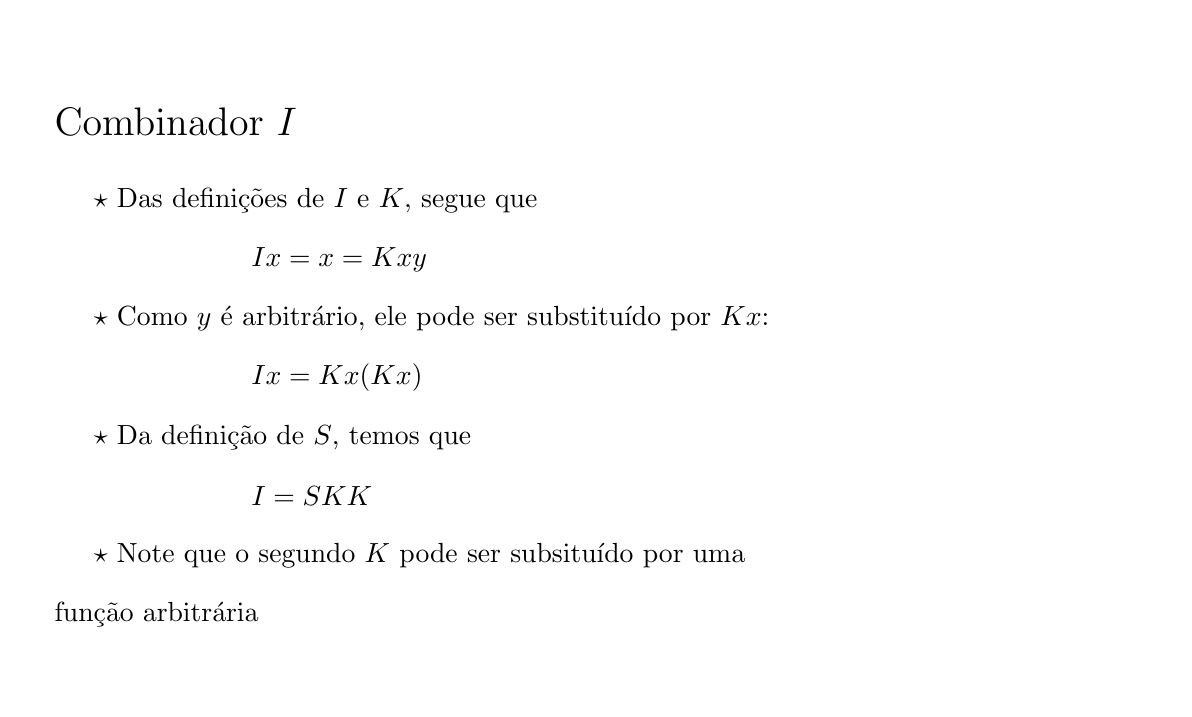
\begin{tikzpicture}
\node[draw,opacity=0] at (0, 0) {x};
\node[draw,opacity=0] at (14, 8) {x};

	\node[anchor=west] (title) at (0.0, 7.0) { \Large \bbbold{Combinador $I$} };


	\node[anchor=west] (a) at (0.5, 6.0) { $\star$ \bbtext{Das definições de $I$ e $K$, segue que} };

	\node[anchor=west] (a1) at (2.5, 5.25) { $Ix = x = Kxy$ };


	\node[anchor=west] (b) at (0.5, 4.5) { $\star$ \bbtext{Como $y$ é arbitrário, ele pode ser substituído por $Kx$:} };

	\node[anchor=west] (b1) at (2.5, 3.75) { $Ix = Kx(Kx)$ };


	\node[anchor=west] (c) at (0.5, 3.0) { $\star$ \bbtext{Da definição de $S$,  temos que} };

	\node[anchor=west] (c1) at (2.5, 2.25) { $I = SKK$ };


	\node[anchor=west] (d) at (0.5, 1.5) { $\star$ \bbtext{Note que o segundo $K$ pode ser subsituído por uma} };

	\node[anchor=west] (d1) at (0.0, 0.75) { \bbtext{função arbitrária} };


\end{tikzpicture}
\end{frame}
\begin{frame}[plain,t]
\begin{tikzpicture}
\node[draw,opacity=0] at (0, 0) {x};
\node[draw,opacity=0] at (14, 8) {x};

	\node[anchor=west] (title) at (0.0, 7.0) { \Large \bbbold{Combinador $I$} };


	\node[anchor=west] (a) at (0.5, 6.0) { $\star$ \bbtext{Das definições de $I$ e $K$, segue que} };

	\node[anchor=west] (a1) at (2.5, 5.25) { $Ix = x = Kxy$ };


	\node[anchor=west] (b) at (0.5, 4.5) { $\star$ \bbtext{Como $y$ é arbitrário, ele pode ser substituído por $Kx$:} };

	\node[anchor=west] (b1) at (2.5, 3.75) { $Ix = Kx(Kx)$ };


	\node[anchor=west] (c) at (0.5, 3.0) { $\star$ \bbtext{Da definição de $S$,  temos que} };

	\node[anchor=west] (c1) at (2.5, 2.25) { $I = SKK$ };


	\node[anchor=west] (d) at (0.5, 1.5) { $\star$ \bbtext{Note que o segundo $K$ pode ser subsituído por uma} };

	\node[anchor=west] (d1) at (0.0, 0.75) { \bbtext{função arbitrária} };



	\node[] (identity) at (12.0, 4.0) { 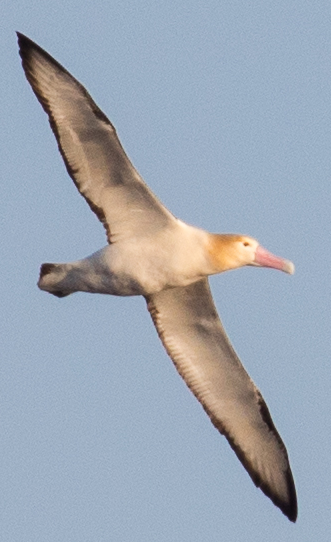
\includegraphics[scale=.3]{figs/identity.png} };

	\node[] (label) at (12.0, 0.75) { \footnotesize \bbtext{Albatroz de cauda curta (\bbenglish{`idiot bird'})} };

\end{tikzpicture}
\end{frame}
\begin{frame}[plain,t]
\begin{tikzpicture}
\node[draw,opacity=0] at (0, 0) {x};
\node[draw,opacity=0] at (14, 8) {x};

	\node[anchor=west] (title) at (0.0, 7.0) { \Large \bbbold{Combinador $B$} };

\end{tikzpicture}
\end{frame}
\begin{frame}[plain,t]
\begin{tikzpicture}
\node[draw,opacity=0] at (0, 0) {x};
\node[draw,opacity=0] at (14, 8) {x};

	\node[anchor=west] (title) at (0.0, 7.0) { \Large \bbbold{Combinador $B$} };


	\node[] (bluebird) at (3.0, 4.5) { 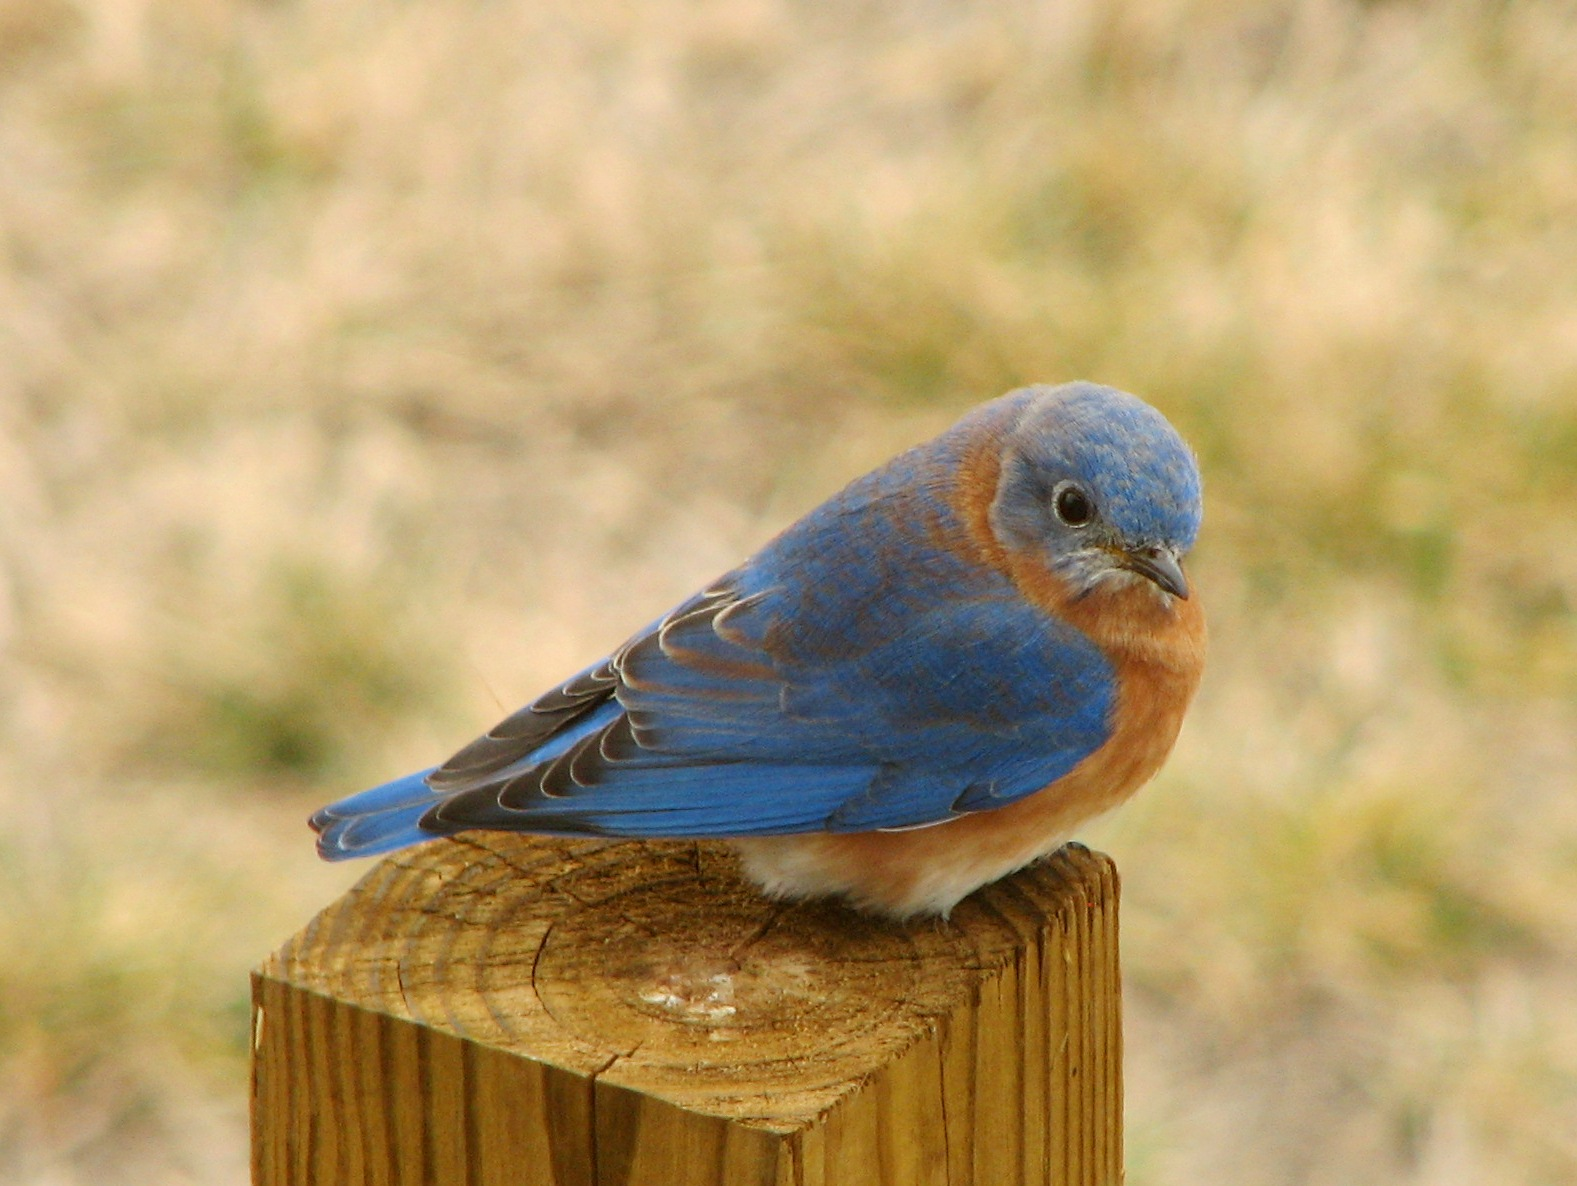
\includegraphics[scale=0.2]{figs/bluebird.jpg} };

	\node[] (label) at (3.0, 2.5) { \footnotesize \bbtext{Tordo-azul-oriental (\bbenglish{bluebird})} };

\end{tikzpicture}
\end{frame}
\begin{frame}[plain,t]
\begin{tikzpicture}
\node[draw,opacity=0] at (0, 0) {x};
\node[draw,opacity=0] at (14, 8) {x};

	\node[anchor=west] (title) at (0.0, 7.0) { \Large \bbbold{Combinador $B$} };


	\node[] (bluebird) at (3.0, 4.5) { 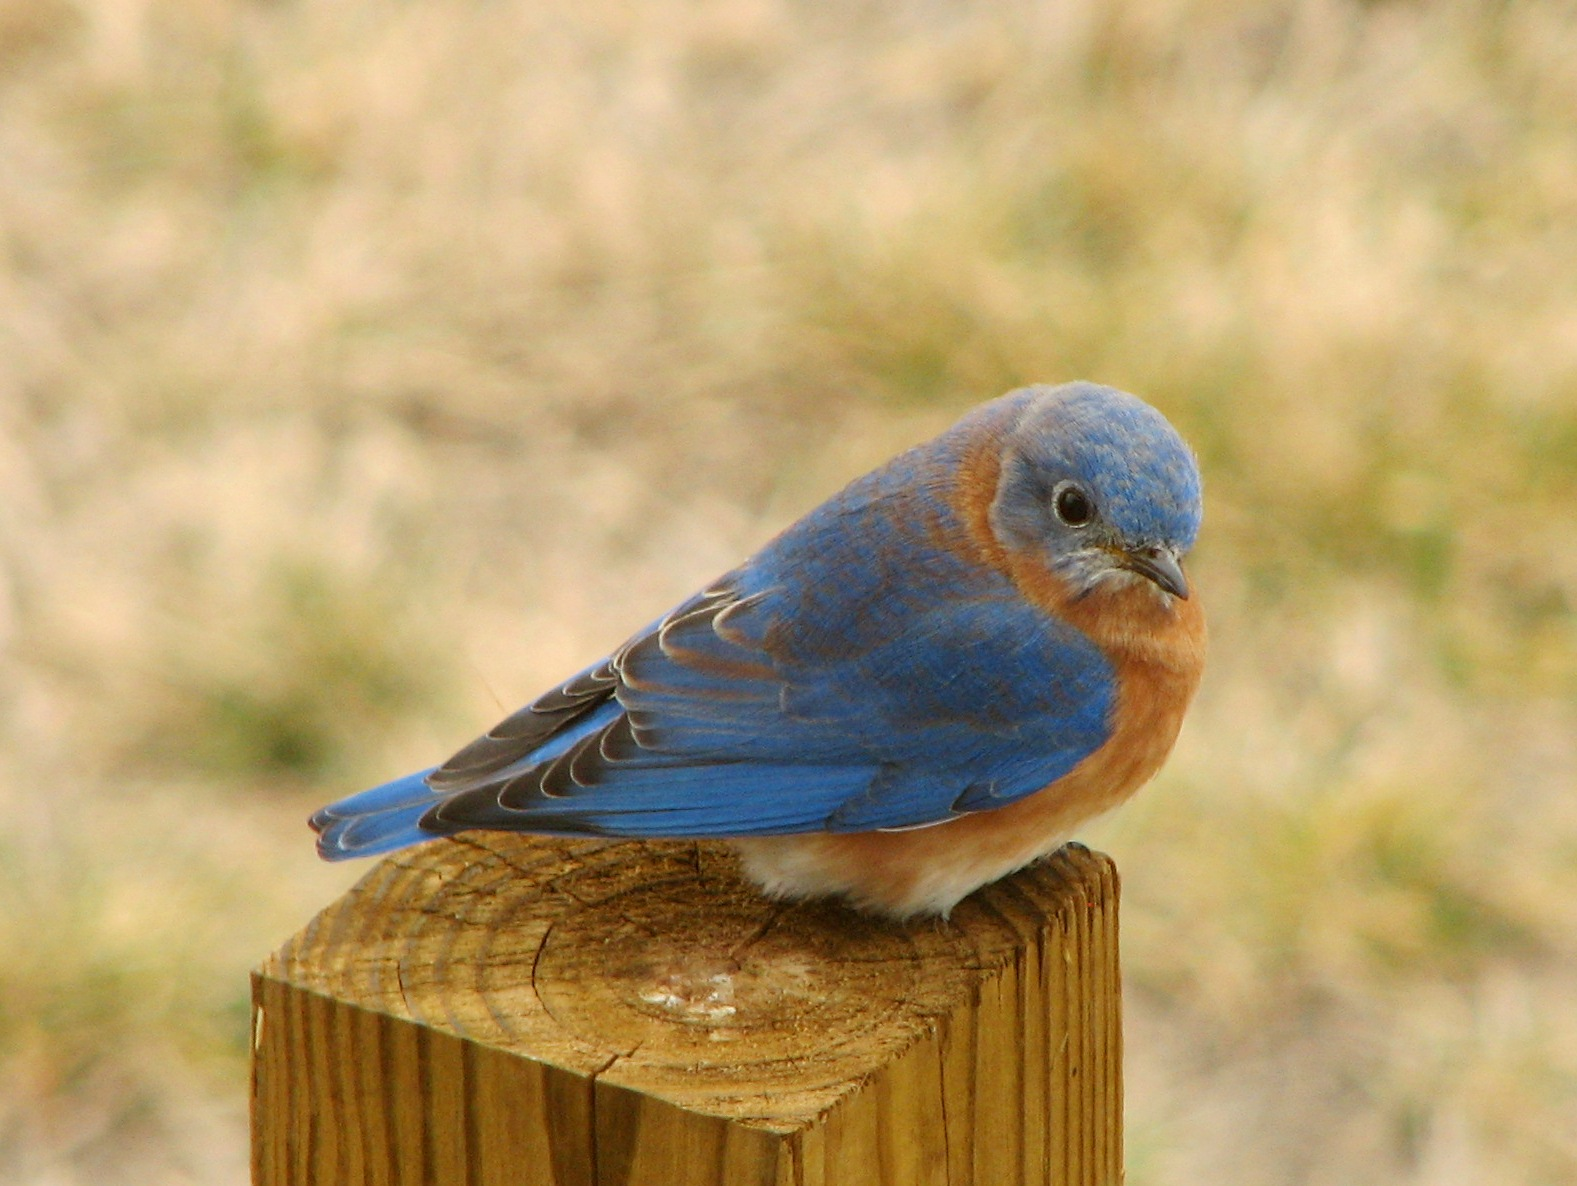
\includegraphics[scale=0.2]{figs/bluebird.jpg} };

	\node[] (label) at (3.0, 2.5) { \footnotesize \bbtext{Tordo-azul-oriental (\bbenglish{bluebird})} };


	\node[anchor=west] (a) at (5.5, 6.0) { $\star$ \bbtext{Representado por Schönfinkel pela letra $Z$} };

\end{tikzpicture}
\end{frame}
\begin{frame}[plain,t]
\begin{tikzpicture}
\node[draw,opacity=0] at (0, 0) {x};
\node[draw,opacity=0] at (14, 8) {x};

	\node[anchor=west] (title) at (0.0, 7.0) { \Large \bbbold{Combinador $B$} };


	\node[] (bluebird) at (3.0, 4.5) { 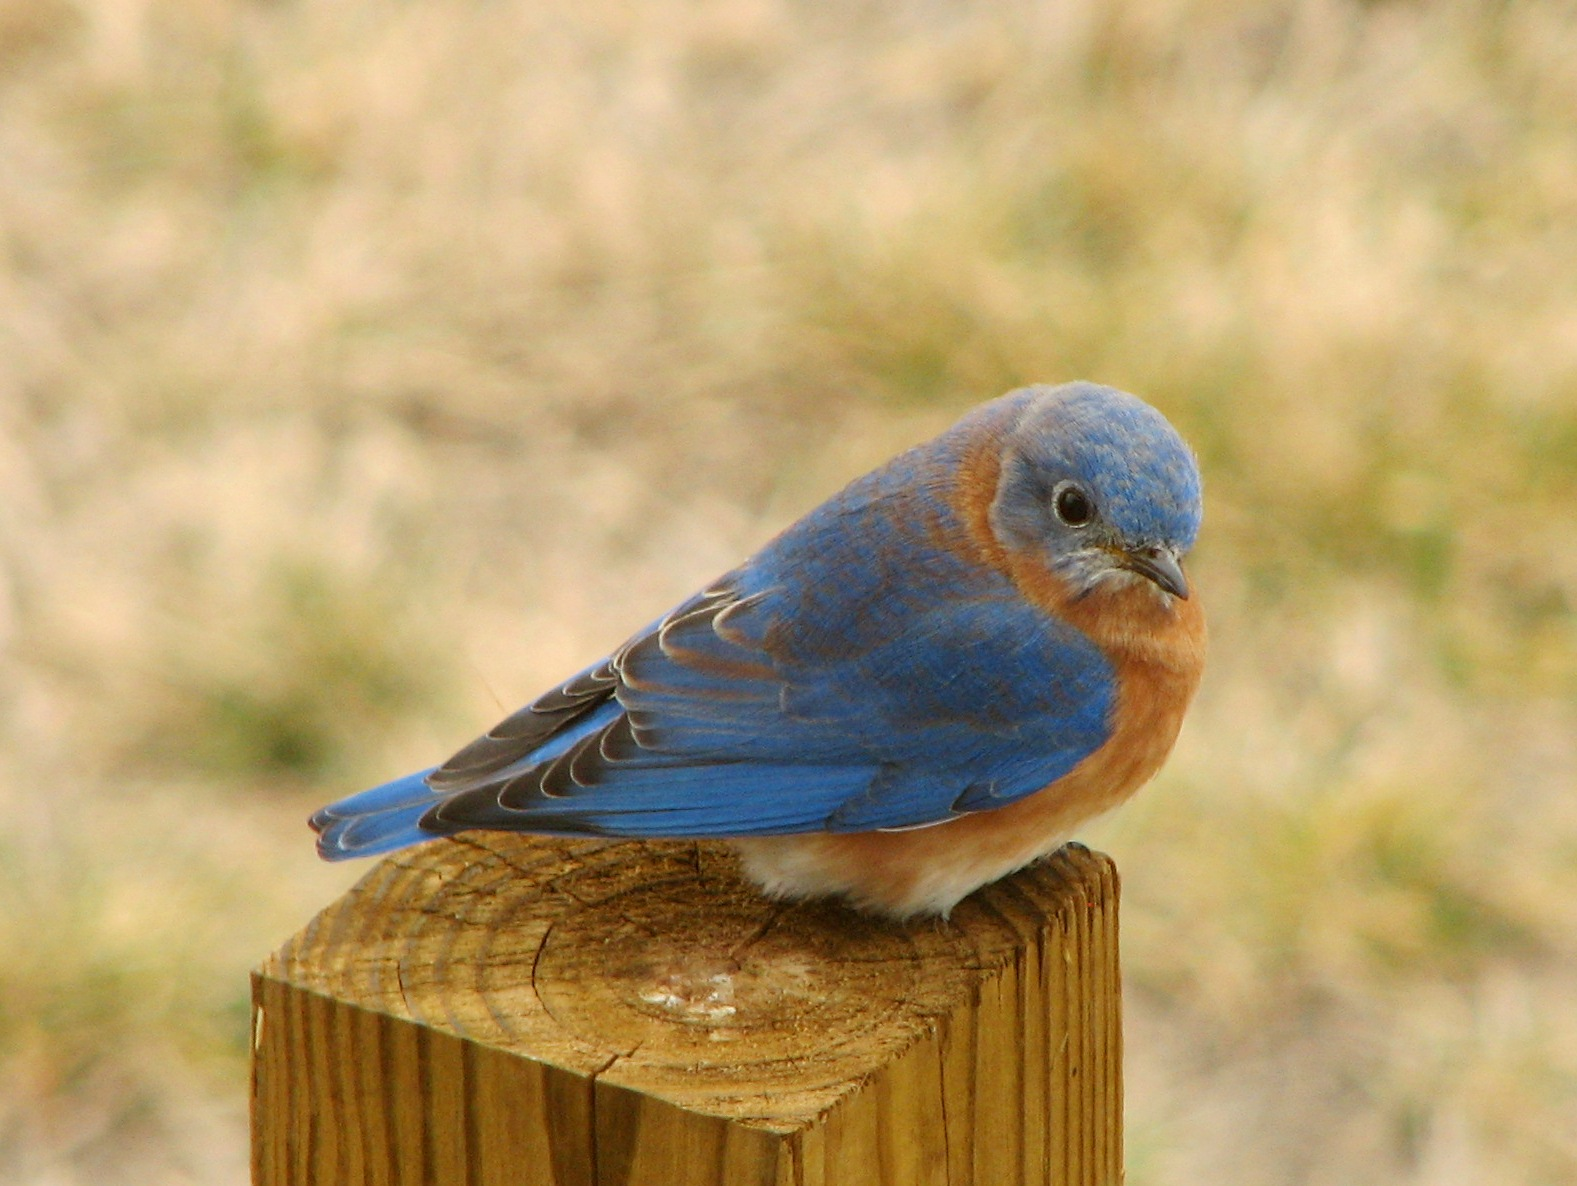
\includegraphics[scale=0.2]{figs/bluebird.jpg} };

	\node[] (label) at (3.0, 2.5) { \footnotesize \bbtext{Tordo-azul-oriental (\bbenglish{bluebird})} };


	\node[anchor=west] (a) at (5.5, 6.0) { $\star$ \bbtext{Representado por Schönfinkel pela letra $Z$} };


	\node[anchor=west] (b) at (5.5, 5.0) { $\star$ \bbtext{Pela definição,} };

	\node[anchor=west] (b1) at (8.0, 4.25) { $Bfgx = f(gx)$ };

\end{tikzpicture}
\end{frame}
\begin{frame}[plain,t]
\begin{tikzpicture}
\node[draw,opacity=0] at (0, 0) {x};
\node[draw,opacity=0] at (14, 8) {x};

	\node[anchor=west] (title) at (0.0, 7.0) { \Large \bbbold{Combinador $B$} };


	\node[] (bluebird) at (3.0, 4.5) { 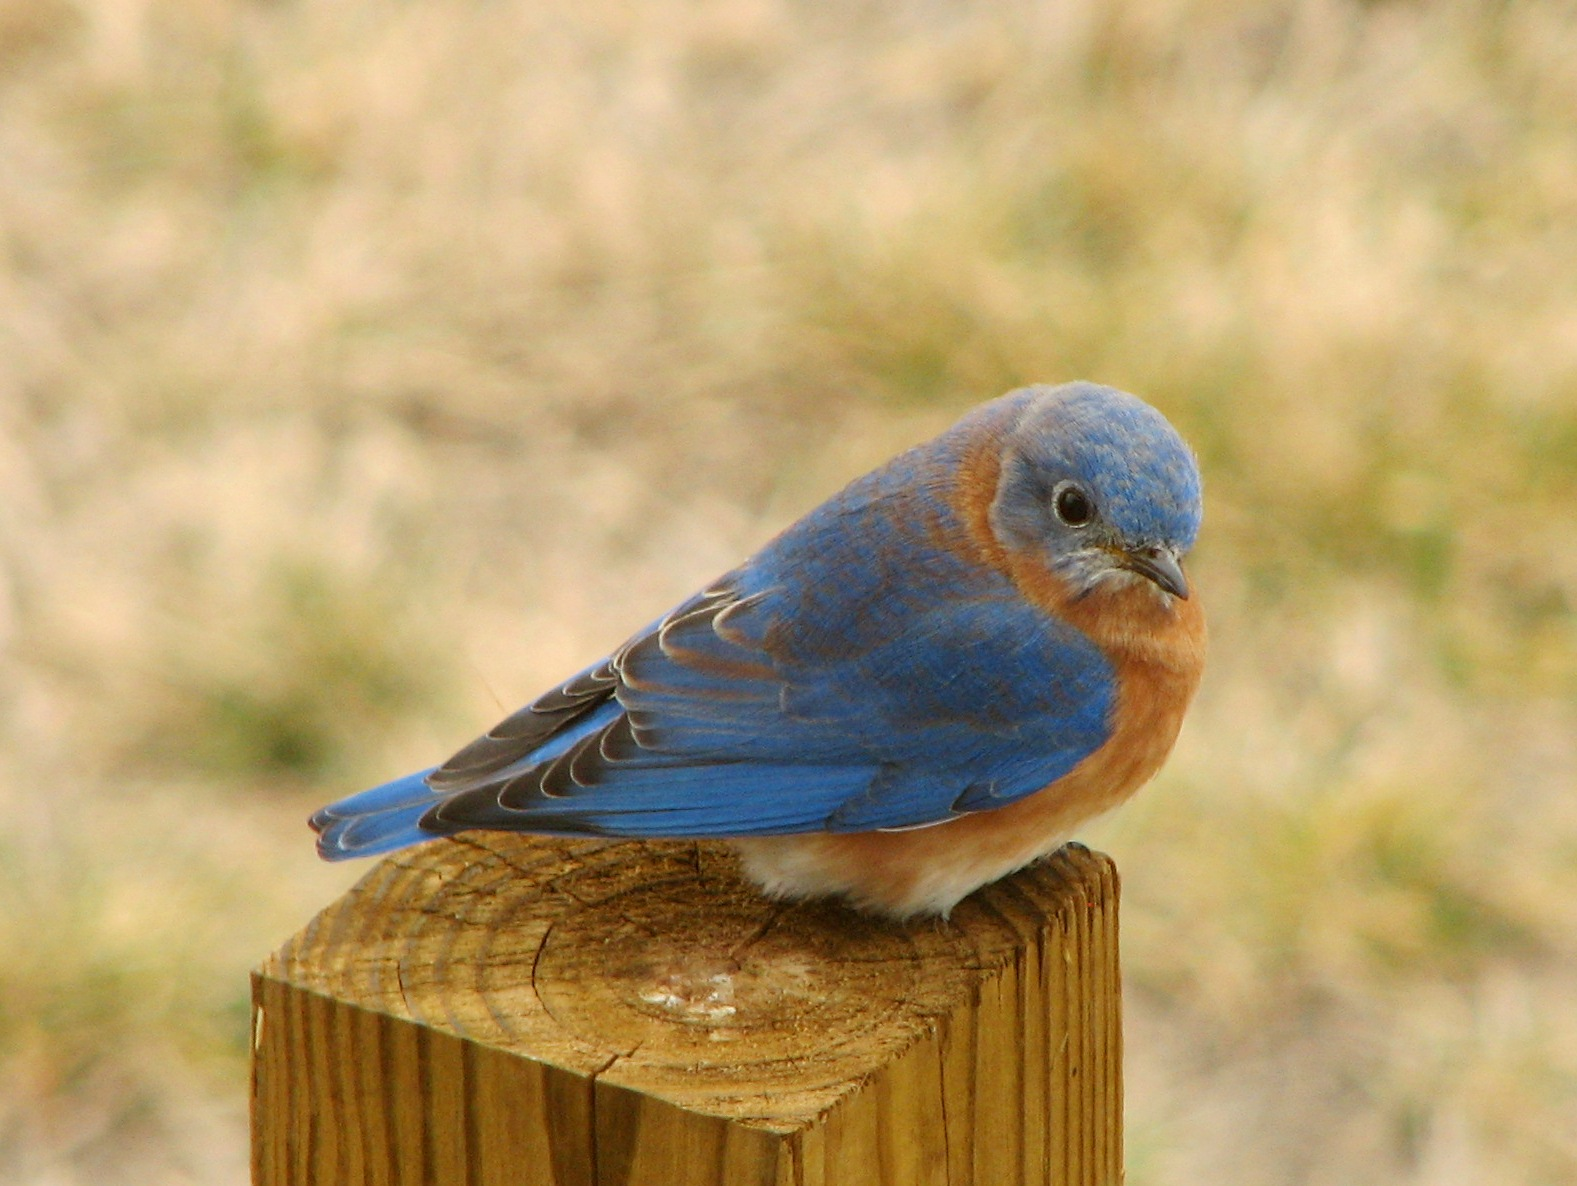
\includegraphics[scale=0.2]{figs/bluebird.jpg} };

	\node[] (label) at (3.0, 2.5) { \footnotesize \bbtext{Tordo-azul-oriental (\bbenglish{bluebird})} };


	\node[anchor=west] (a) at (5.5, 6.0) { $\star$ \bbtext{Representado por Schönfinkel pela letra $Z$} };


	\node[anchor=west] (b) at (5.5, 5.0) { $\star$ \bbtext{Pela definição,} };

	\node[anchor=west] (b1) at (8.0, 4.25) { $Bfgx = f(gx)$ };


	\node[anchor=west] (c) at (5.5, 3.5) { $\star$ \bbtext{Observe que} };

	\node[anchor=west] (c1) at (6.0, 2.75) { $f(gx) = (Kfx)(gx) = S(Kf)gx = (KSf)(Kf)gx$ };

\end{tikzpicture}
\end{frame}
\begin{frame}[plain,t]
\begin{tikzpicture}
\node[draw,opacity=0] at (0, 0) {x};
\node[draw,opacity=0] at (14, 8) {x};

	\node[anchor=west] (title) at (0.0, 7.0) { \Large \bbbold{Combinador $B$} };


	\node[] (bluebird) at (3.0, 4.5) { 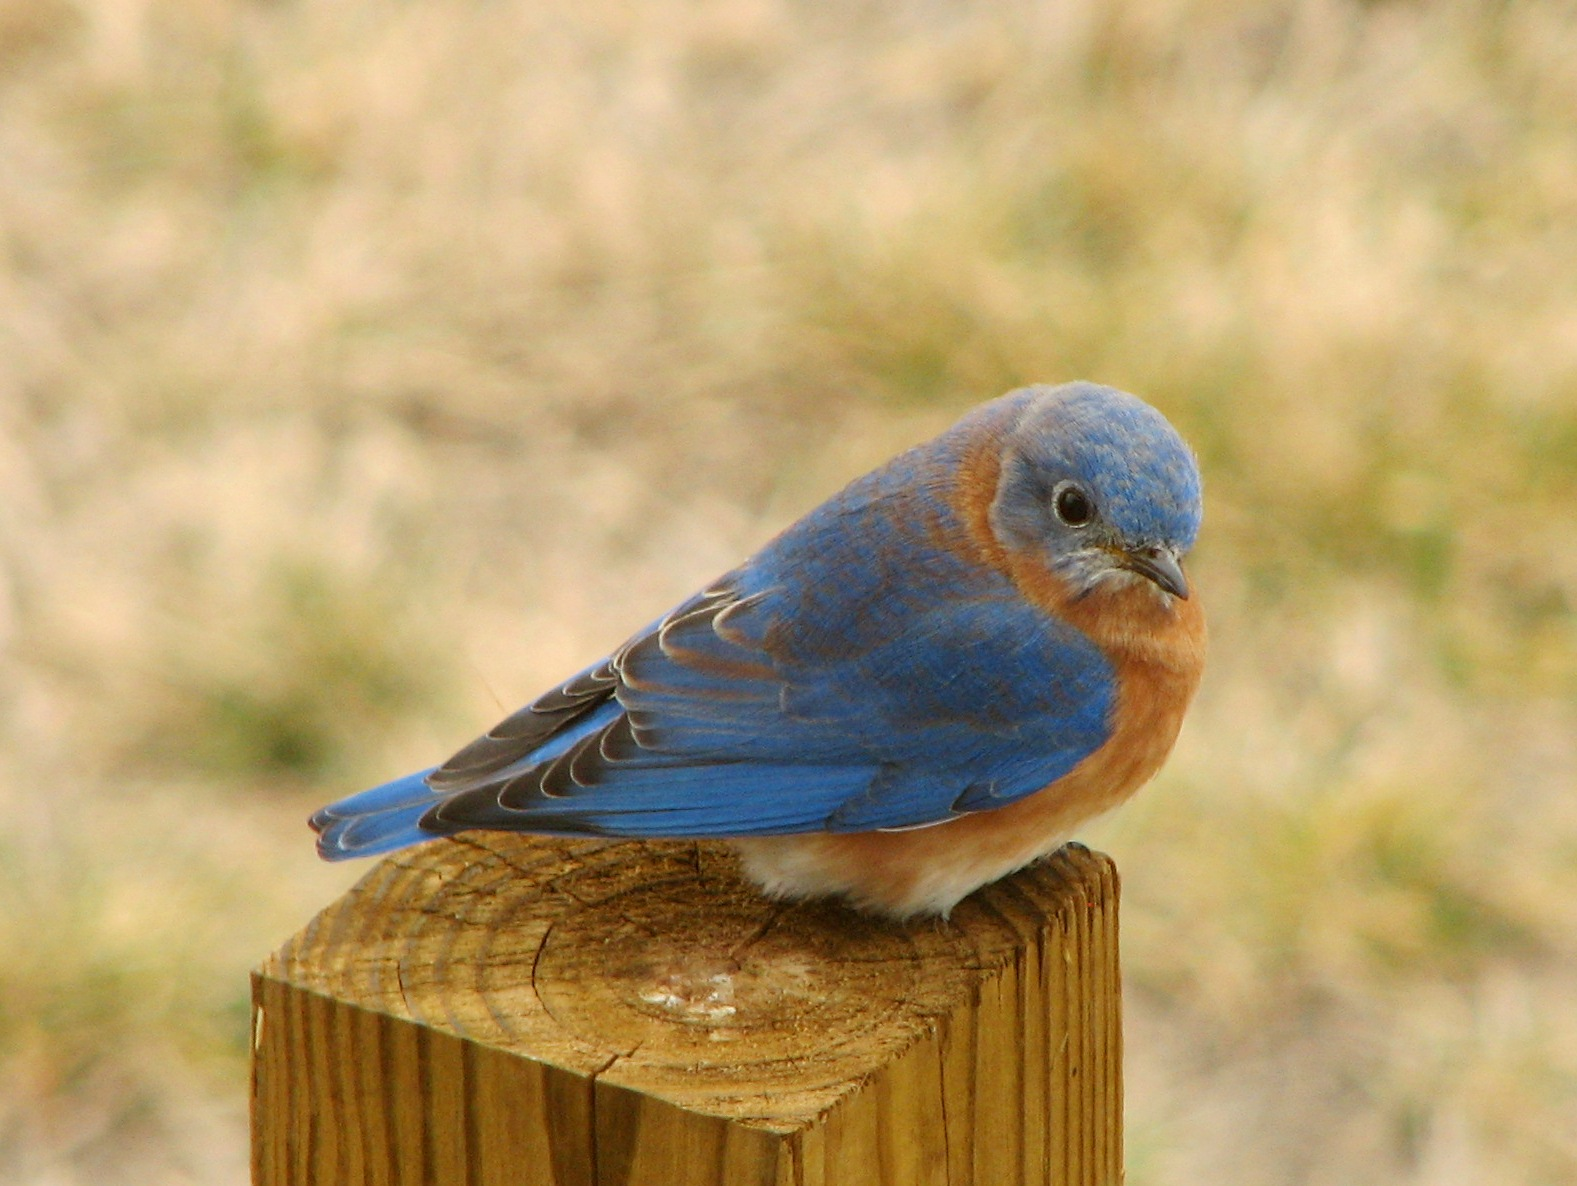
\includegraphics[scale=0.2]{figs/bluebird.jpg} };

	\node[] (label) at (3.0, 2.5) { \footnotesize \bbtext{Tordo-azul-oriental (\bbenglish{bluebird})} };


	\node[anchor=west] (a) at (5.5, 6.0) { $\star$ \bbtext{Representado por Schönfinkel pela letra $Z$} };


	\node[anchor=west] (b) at (5.5, 5.0) { $\star$ \bbtext{Pela definição,} };

	\node[anchor=west] (b1) at (8.0, 4.25) { $Bfgx = f(gx)$ };


	\node[anchor=west] (c) at (5.5, 3.5) { $\star$ \bbtext{Observe que} };

	\node[anchor=west] (c1) at (6.0, 2.75) { $f(gx) = (Kfx)(gx) = S(Kf)gx = (KSf)(Kf)gx$ };


	\node[anchor=west] (d) at (5.5, 2.0) { $\star$ \bbtext{Uma nova fusão em $f$ nos leva a} };

	\node[anchor=west] (d1) at (8.0, 1.25) { $f(gx) = S(KS)Kfgx$ };

\end{tikzpicture}
\end{frame}
\begin{frame}[plain,t]
\begin{tikzpicture}
\node[draw,opacity=0] at (0, 0) {x};
\node[draw,opacity=0] at (14, 8) {x};

	\node[anchor=west] (title) at (0.0, 7.0) { \Large \bbbold{Combinador $B$} };


	\node[] (bluebird) at (3.0, 4.5) { 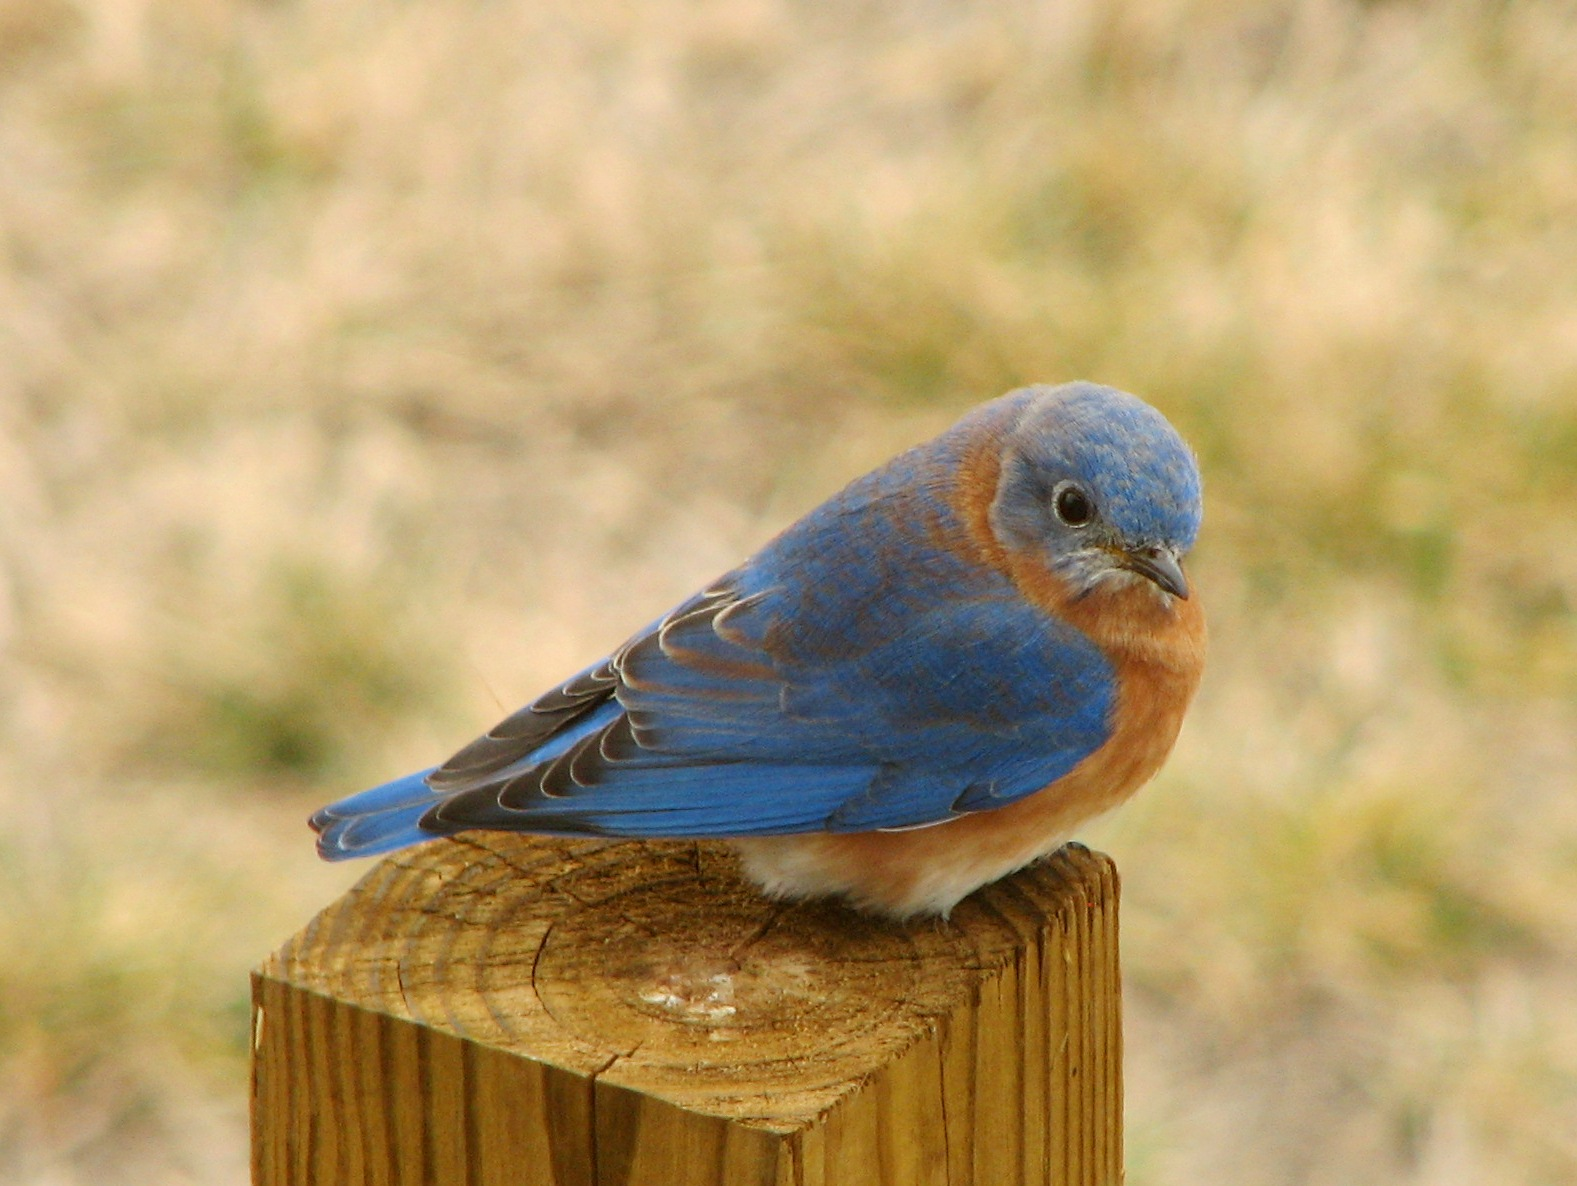
\includegraphics[scale=0.2]{figs/bluebird.jpg} };

	\node[] (label) at (3.0, 2.5) { \footnotesize \bbtext{Tordo-azul-oriental (\bbenglish{bluebird})} };


	\node[anchor=west] (a) at (5.5, 6.0) { $\star$ \bbtext{Representado por Schönfinkel pela letra $Z$} };


	\node[anchor=west] (b) at (5.5, 5.0) { $\star$ \bbtext{Pela definição,} };

	\node[anchor=west] (b1) at (8.0, 4.25) { $Bfgx = f(gx)$ };


	\node[anchor=west] (c) at (5.5, 3.5) { $\star$ \bbtext{Observe que} };

	\node[anchor=west] (c1) at (6.0, 2.75) { $f(gx) = (Kfx)(gx) = S(Kf)gx = (KSf)(Kf)gx$ };


	\node[anchor=west] (d) at (5.5, 2.0) { $\star$ \bbtext{Uma nova fusão em $f$ nos leva a} };

	\node[anchor=west] (d1) at (8.0, 1.25) { $f(gx) = S(KS)Kfgx$ };


	\node[anchor=west] (e) at (5.5, 0.5) { $\star$ \bbtext{Portanto, $B = S(KS)K$} };

\end{tikzpicture}
\end{frame}
\begin{frame}[plain,t]
\begin{tikzpicture}
\node[draw,opacity=0] at (0, 0) {x};
\node[draw,opacity=0] at (14, 8) {x};

	\node[anchor=west] (title) at (0.0, 7.0) { \Large \bbbold{Combinador $C$} };

\end{tikzpicture}
\end{frame}
\begin{frame}[plain,t]
\begin{tikzpicture}
\node[draw,opacity=0] at (0, 0) {x};
\node[draw,opacity=0] at (14, 8) {x};

	\node[anchor=west] (title) at (0.0, 7.0) { \Large \bbbold{Combinador $C$} };

	\node[] (cardinal) at (12.0, 4.0) { 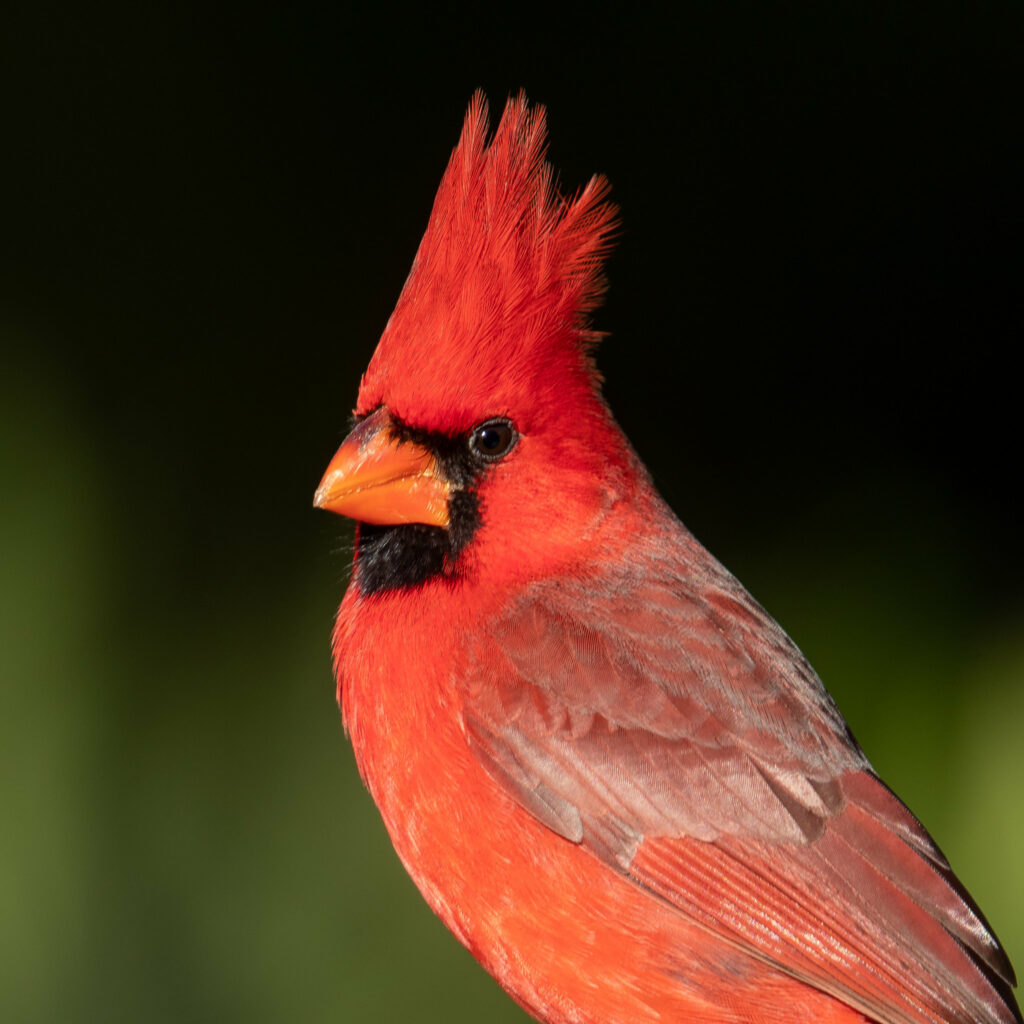
\includegraphics[scale=0.125]{figs/cardinal.jpg} };

	\node[] (label) at (12.0, 1.25) { \footnotesize \bbtext{Cardeal-do-norte (\bbenglish{cardinal})} };

	\node[anchor=west] (a) at (0.5, 6.0) { $\star$ \bbtext{Corresponde ao combinador $T$ de Schönfinkel} };

\end{tikzpicture}
\end{frame}
\begin{frame}[plain,t]
\begin{tikzpicture}
\node[draw,opacity=0] at (0, 0) {x};
\node[draw,opacity=0] at (14, 8) {x};

	\node[anchor=west] (title) at (0.0, 7.0) { \Large \bbbold{Combinador $C$} };

	\node[] (cardinal) at (12.0, 4.0) { 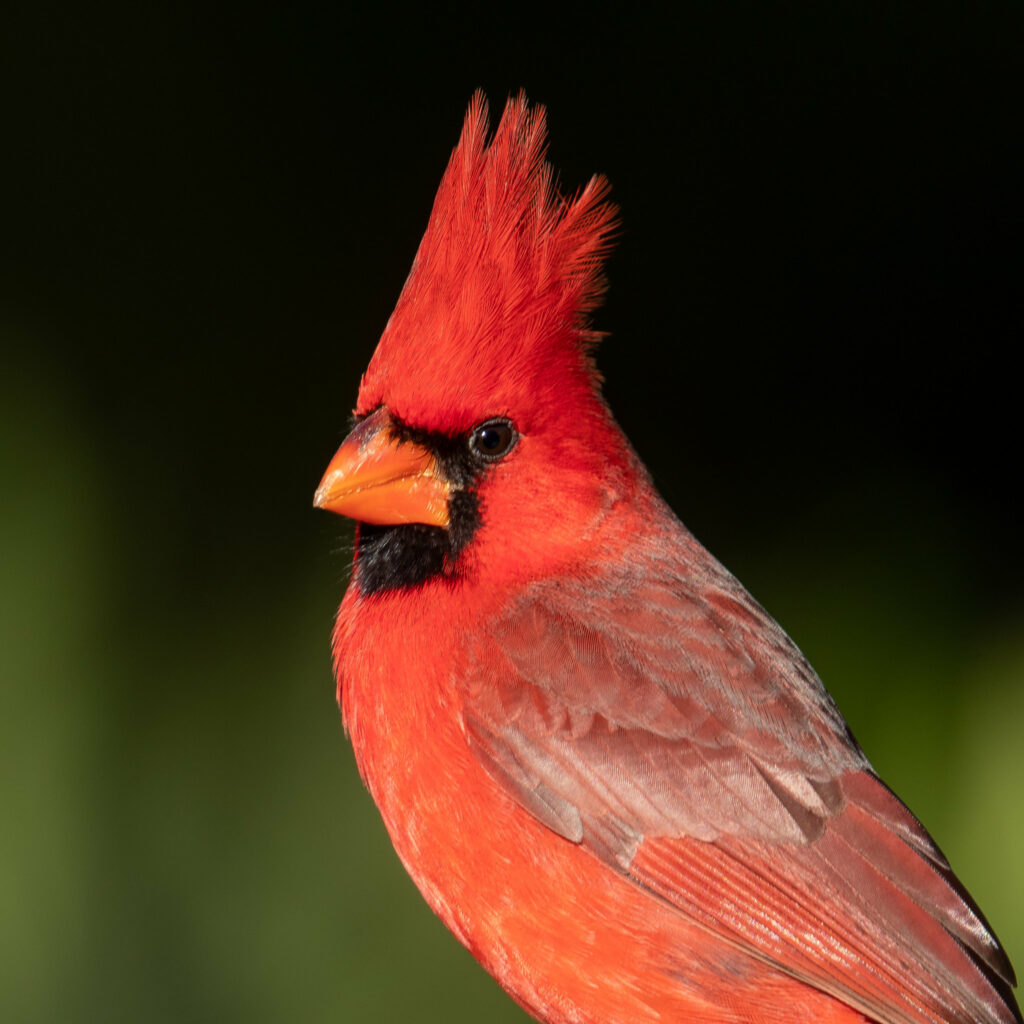
\includegraphics[scale=0.125]{figs/cardinal.jpg} };

	\node[] (label) at (12.0, 1.25) { \footnotesize \bbtext{Cardeal-do-norte (\bbenglish{cardinal})} };

	\node[anchor=west] (a) at (0.5, 6.0) { $\star$ \bbtext{Corresponde ao combinador $T$ de Schönfinkel} };


	\node[anchor=west] (b) at (0.5, 5.0) { $\star$ \bbtext{Vale a seguinte sequência de transformações:} };

	\node[anchor=west] (b1) at (1.25, 4.0) { $fxy = fx(Kyx) = (fx)(Kyx) = Sf(Ky)x$ };

	\node[anchor=west] (b2) at (2.0, 3.25) { $= (Sf)(Ky)x = B(Sf)Kyx$ };

	\node[anchor=west] (b3) at (2.0, 2.5) { $= BBSfKyx = (BBSf)Kyx$ };

	\node[anchor=west] (b4) at (2.0, 1.75) { $= (BBSf)(KKf)yx = S(BBS)(KK)fyx$ };

\end{tikzpicture}
\end{frame}
\begin{frame}[plain,t]
\begin{tikzpicture}
\node[draw,opacity=0] at (0, 0) {x};
\node[draw,opacity=0] at (14, 8) {x};

	\node[anchor=west] (title) at (0.0, 7.0) { \Large \bbbold{Combinador $C$} };

	\node[] (cardinal) at (12.0, 4.0) { 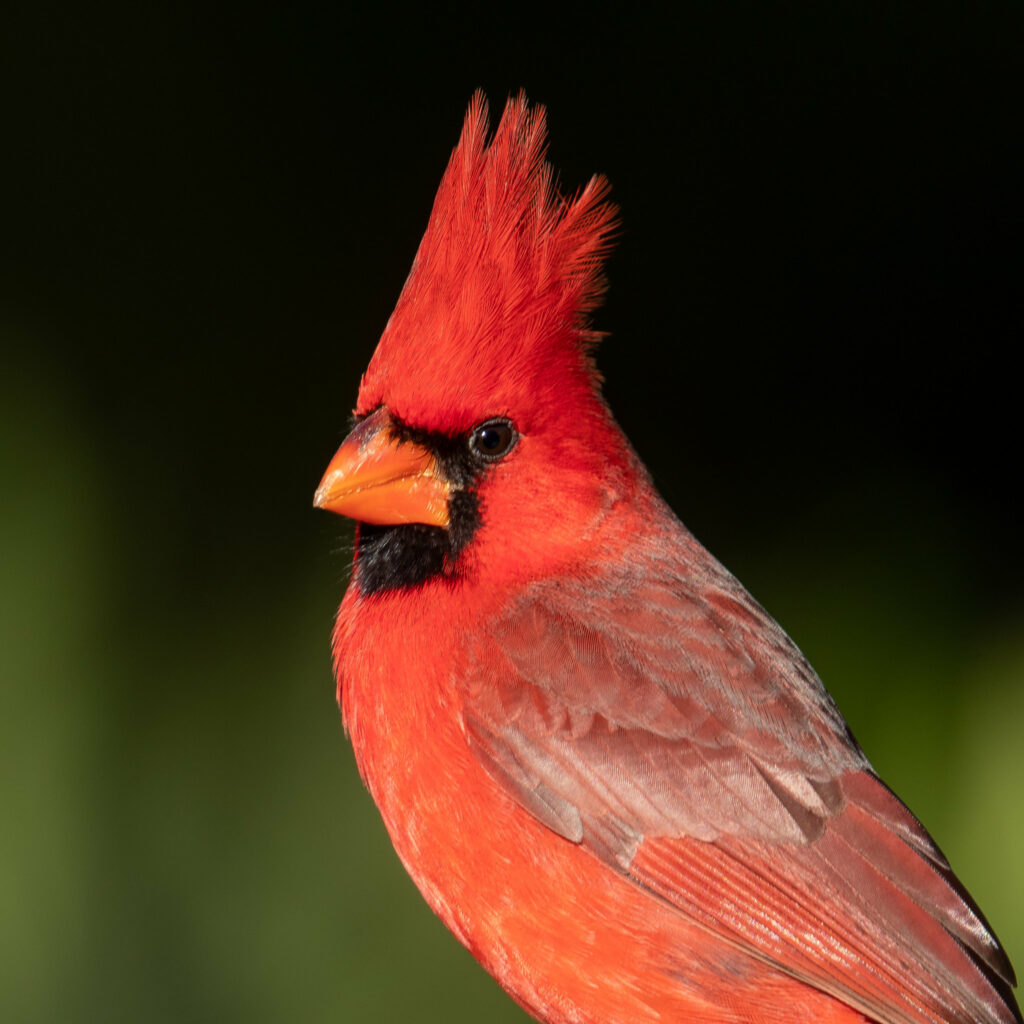
\includegraphics[scale=0.125]{figs/cardinal.jpg} };

	\node[] (label) at (12.0, 1.25) { \footnotesize \bbtext{Cardeal-do-norte (\bbenglish{cardinal})} };

	\node[anchor=west] (a) at (0.5, 6.0) { $\star$ \bbtext{Corresponde ao combinador $T$ de Schönfinkel} };


	\node[anchor=west] (b) at (0.5, 5.0) { $\star$ \bbtext{Vale a seguinte sequência de transformações:} };

	\node[anchor=west] (b1) at (1.25, 4.0) { $fxy = fx(Kyx) = (fx)(Kyx) = Sf(Ky)x$ };

	\node[anchor=west] (b2) at (2.0, 3.25) { $= (Sf)(Ky)x = B(Sf)Kyx$ };

	\node[anchor=west] (b3) at (2.0, 2.5) { $= BBSfKyx = (BBSf)Kyx$ };

	\node[anchor=west] (b4) at (2.0, 1.75) { $= (BBSf)(KKf)yx = S(BBS)(KK)fyx$ };

	\node[anchor=west] (c) at (0.5, 0.7) { $\star$ \bbtext{Portanto, $C = S(BBS)(KK)$} };

\end{tikzpicture}
\end{frame}
\begin{frame}[plain,t]
\vspace*{\fill}

\begin{tikzpicture}
\node[draw,opacity=0] at (0, 0) {x};
\node[draw,opacity=0] at (14, 8) {x};
\node[anchor=west] (title) at (0.0, 7.0) { \Large \bbbold{Função de imcompatibilidade $U$} };

\node[anchor=west] at (0, 3.5) {\begin{tcolorbox}[colback=blue!5,colframe=blue!60!green,title=\textbf{Funções de incompatibilidade}]
\bbtext{O conectivo fundamental de Schönfinkel
$$
fx\ |^x\ gx,
$$
depende de duas funções proposicionais de um argumento $f$ e $g$, logo tem forma $U(f, g)$. Assim, usando a transformação de funções de múltiplos argumentos,
$$
Ufg = fx\ |^x\ gx,
$$
é a equação que define a função de incompatibilidade $U$.}
\end{tcolorbox}};

\end{tikzpicture}

\vspace*{\fill}
\end{frame}
\begin{frame}[plain,t]
\begin{tikzpicture}
\node[draw,opacity=0] at (0, 0) {x};
\node[draw,opacity=0] at (14, 8) {x};

	\node[anchor=west] (title) at (0.0, 7.0) { \Large \bbbold{Principais resultados do artigo} };

\end{tikzpicture}
\end{frame}
\begin{frame}[plain,t]
\begin{tikzpicture}
\node[draw,opacity=0] at (0, 0) {x};
\node[draw,opacity=0] at (14, 8) {x};

	\node[anchor=west] (title) at (0.0, 7.0) { \Large \bbbold{Principais resultados do artigo} };


	\node[anchor=west] (a) at (1.0, 6.0) { $\star$ \bbtext{Schönfinkel afirma que qualquer fórmula lógica de primeira ordem pode ser } };

	\node[anchor=west] (a1) at (0.5, 5.5) { \bbtext{expressa em termos das funções particulares $I, C, T, Z, S$ e $U$.} };

\end{tikzpicture}
\end{frame}
\begin{frame}[plain,t]
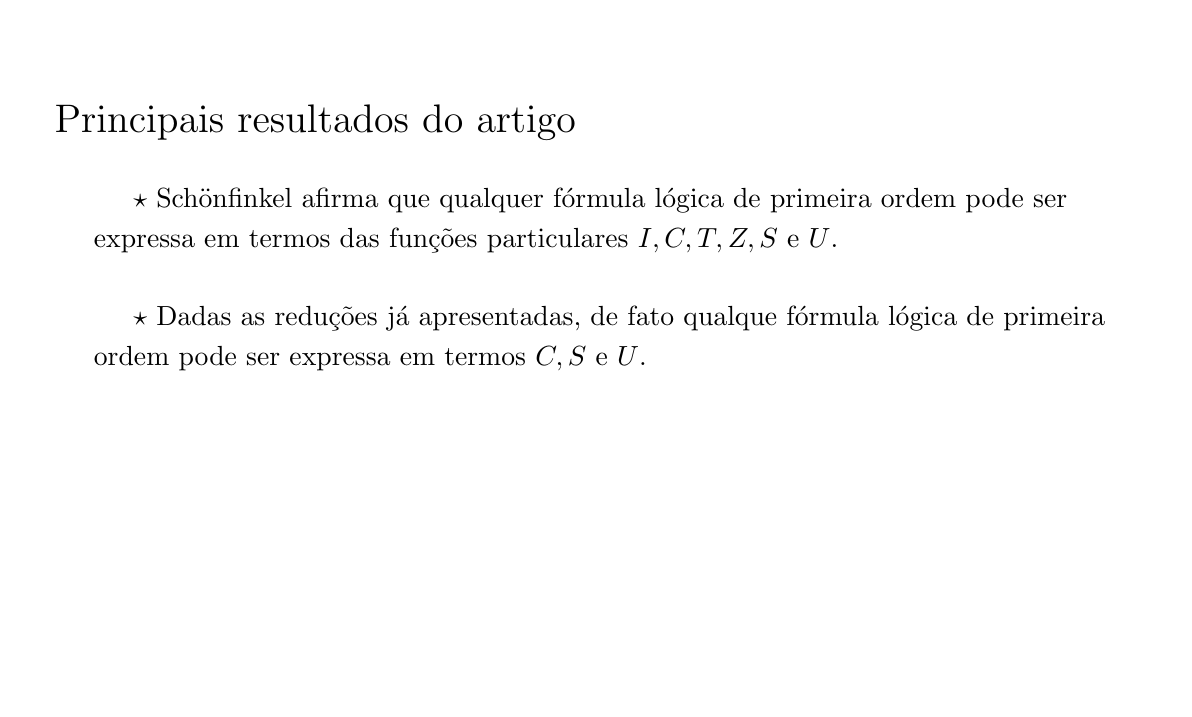
\begin{tikzpicture}
\node[draw,opacity=0] at (0, 0) {x};
\node[draw,opacity=0] at (14, 8) {x};

	\node[anchor=west] (title) at (0.0, 7.0) { \Large \bbbold{Principais resultados do artigo} };


	\node[anchor=west] (a) at (1.0, 6.0) { $\star$ \bbtext{Schönfinkel afirma que qualquer fórmula lógica de primeira ordem pode ser } };

	\node[anchor=west] (a1) at (0.5, 5.5) { \bbtext{expressa em termos das funções particulares $I, C, T, Z, S$ e $U$.} };


	\node[anchor=west] (b) at (1.0, 4.5) { $\star$ \bbtext{Dadas as reduções já apresentadas, de fato qualque fórmula lógica de primeira} };

	\node[anchor=west] (b1) at (0.5, 4.0) { \bbtext{ordem pode ser expressa em termos $C, S$ e $U$.} };

\end{tikzpicture}
\end{frame}
\begin{frame}[plain,t]
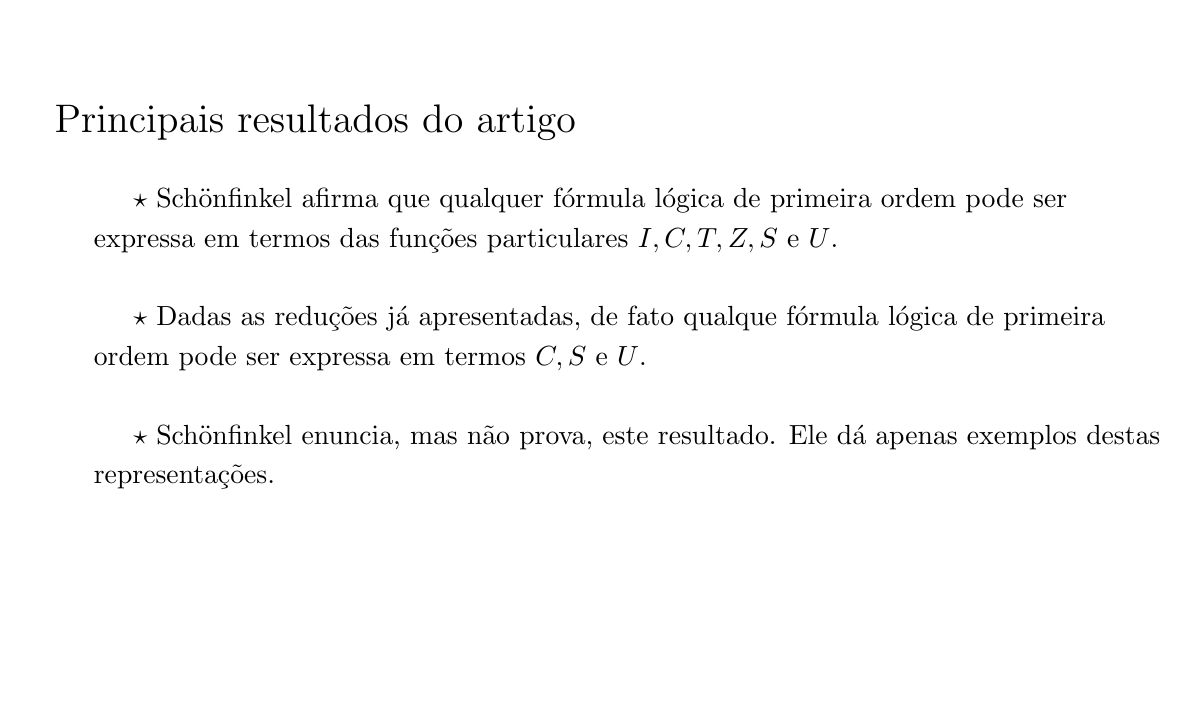
\begin{tikzpicture}
\node[draw,opacity=0] at (0, 0) {x};
\node[draw,opacity=0] at (14, 8) {x};

	\node[anchor=west] (title) at (0.0, 7.0) { \Large \bbbold{Principais resultados do artigo} };


	\node[anchor=west] (a) at (1.0, 6.0) { $\star$ \bbtext{Schönfinkel afirma que qualquer fórmula lógica de primeira ordem pode ser } };

	\node[anchor=west] (a1) at (0.5, 5.5) { \bbtext{expressa em termos das funções particulares $I, C, T, Z, S$ e $U$.} };


	\node[anchor=west] (b) at (1.0, 4.5) { $\star$ \bbtext{Dadas as reduções já apresentadas, de fato qualque fórmula lógica de primeira} };

	\node[anchor=west] (b1) at (0.5, 4.0) { \bbtext{ordem pode ser expressa em termos $C, S$ e $U$.} };


	\node[anchor=west] (c) at (1.0, 3.0) { $\star$ \bbtext{Schönfinkel enuncia, mas não prova, este resultado. Ele dá apenas exemplos destas} };

	\node[anchor=west] (c1) at (0.5, 2.5) { \bbtext{representações.} };

\end{tikzpicture}
\end{frame}
\begin{frame}[plain,t]
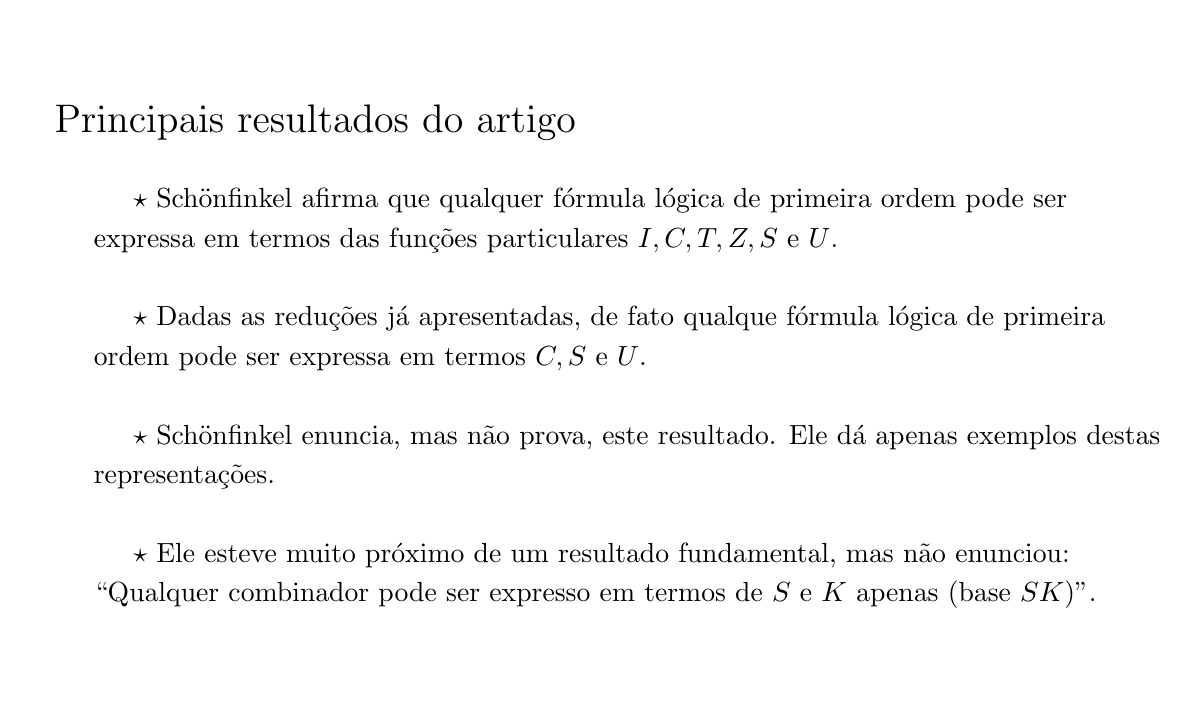
\begin{tikzpicture}
\node[draw,opacity=0] at (0, 0) {x};
\node[draw,opacity=0] at (14, 8) {x};

	\node[anchor=west] (title) at (0.0, 7.0) { \Large \bbbold{Principais resultados do artigo} };


	\node[anchor=west] (a) at (1.0, 6.0) { $\star$ \bbtext{Schönfinkel afirma que qualquer fórmula lógica de primeira ordem pode ser } };

	\node[anchor=west] (a1) at (0.5, 5.5) { \bbtext{expressa em termos das funções particulares $I, C, T, Z, S$ e $U$.} };


	\node[anchor=west] (b) at (1.0, 4.5) { $\star$ \bbtext{Dadas as reduções já apresentadas, de fato qualque fórmula lógica de primeira} };

	\node[anchor=west] (b1) at (0.5, 4.0) { \bbtext{ordem pode ser expressa em termos $C, S$ e $U$.} };


	\node[anchor=west] (c) at (1.0, 3.0) { $\star$ \bbtext{Schönfinkel enuncia, mas não prova, este resultado. Ele dá apenas exemplos destas} };

	\node[anchor=west] (c1) at (0.5, 2.5) { \bbtext{representações.} };


	\node[anchor=west] (d) at (1.0, 1.5) { $\star$ \bbtext{Ele esteve muito próximo de um resultado fundamental, mas não enunciou:} };

	\node[anchor=west] (d1) at (0.5, 1.0) { \bbtext{``Qualquer combinador pode ser expresso em termos de $S$ e $K$ apenas (base $SK$)''.} };

\end{tikzpicture}
\end{frame}
\begin{frame}[plain,t]
\begin{tikzpicture}
\node[draw,opacity=0] at (0, 0) {x};
\node[draw,opacity=0] at (14, 8) {x};

	\node[anchor=west] (title) at (0.0, 7.0) { \Large \bbbold{Principais resultados do artigo} };

\end{tikzpicture}
\end{frame}
\begin{frame}[plain,t]
\begin{tikzpicture}
\node[draw,opacity=0] at (0, 0) {x};
\node[draw,opacity=0] at (14, 8) {x};

	\node[anchor=west] (title) at (0.0, 7.0) { \Large \bbbold{Principais resultados do artigo} };


	\node[anchor=west] (a) at (1.0, 6.0) { $\star$ \bbtext{Na útlima seção, Schönfinkel introduz a função $J$, definida pelas igualdades} };

	\node[] (a1) at (7.0, 5.0) { $JC = U,\ \ \ JS = C, \ \ \ \mbox{e}\ \ \ Jx = S$, };

	\node[anchor=west] (a2) at (0.5, 4.25) { \bbtext{onde $x$ é qualquer termo diferente de $C$ e $S$.} };

\end{tikzpicture}
\end{frame}
\begin{frame}[plain,t]
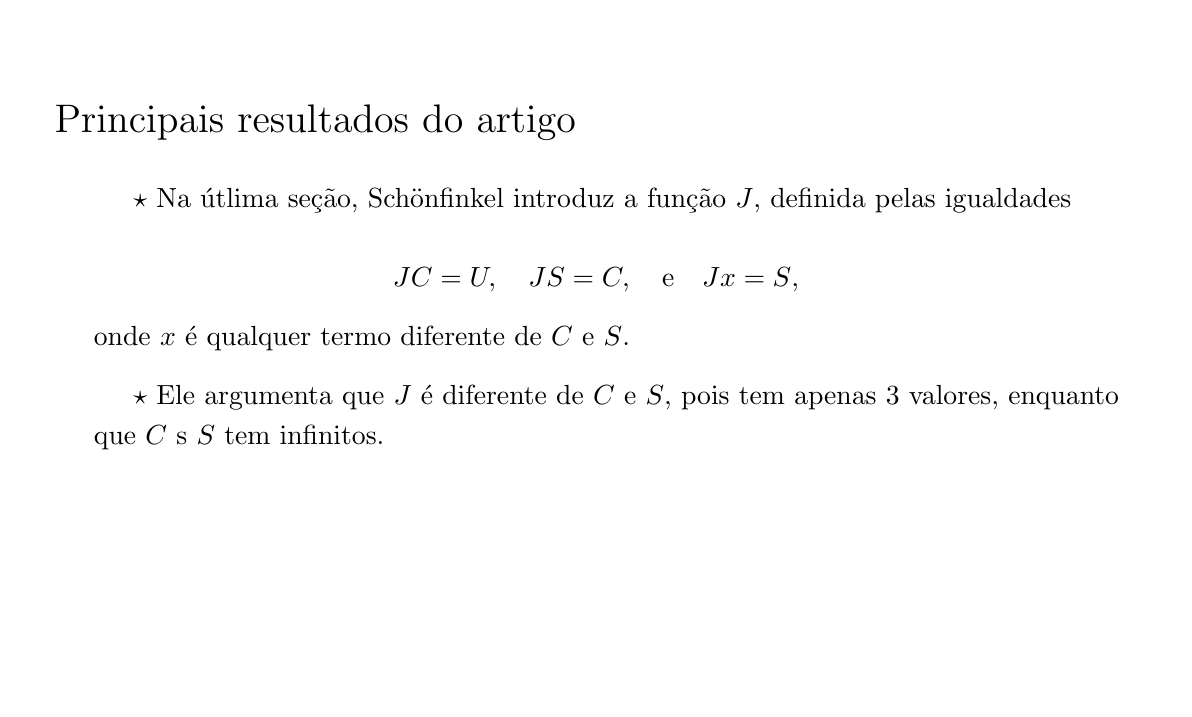
\begin{tikzpicture}
\node[draw,opacity=0] at (0, 0) {x};
\node[draw,opacity=0] at (14, 8) {x};

	\node[anchor=west] (title) at (0.0, 7.0) { \Large \bbbold{Principais resultados do artigo} };


	\node[anchor=west] (a) at (1.0, 6.0) { $\star$ \bbtext{Na útlima seção, Schönfinkel introduz a função $J$, definida pelas igualdades} };

	\node[] (a1) at (7.0, 5.0) { $JC = U,\ \ \ JS = C, \ \ \ \mbox{e}\ \ \ Jx = S$, };

	\node[anchor=west] (a2) at (0.5, 4.25) { \bbtext{onde $x$ é qualquer termo diferente de $C$ e $S$.} };


	\node[anchor=west] (b) at (1.0, 3.5) { $\star$ \bbtext{Ele argumenta que $J$ é diferente de $C$ e $S$, pois tem apenas 3 valores, enquanto} };

	\node[anchor=west] (b1) at (0.5, 3.0) { \bbtext{que $C$ s $S$ tem infinitos.} };

\end{tikzpicture}
\end{frame}
\begin{frame}[plain,t]
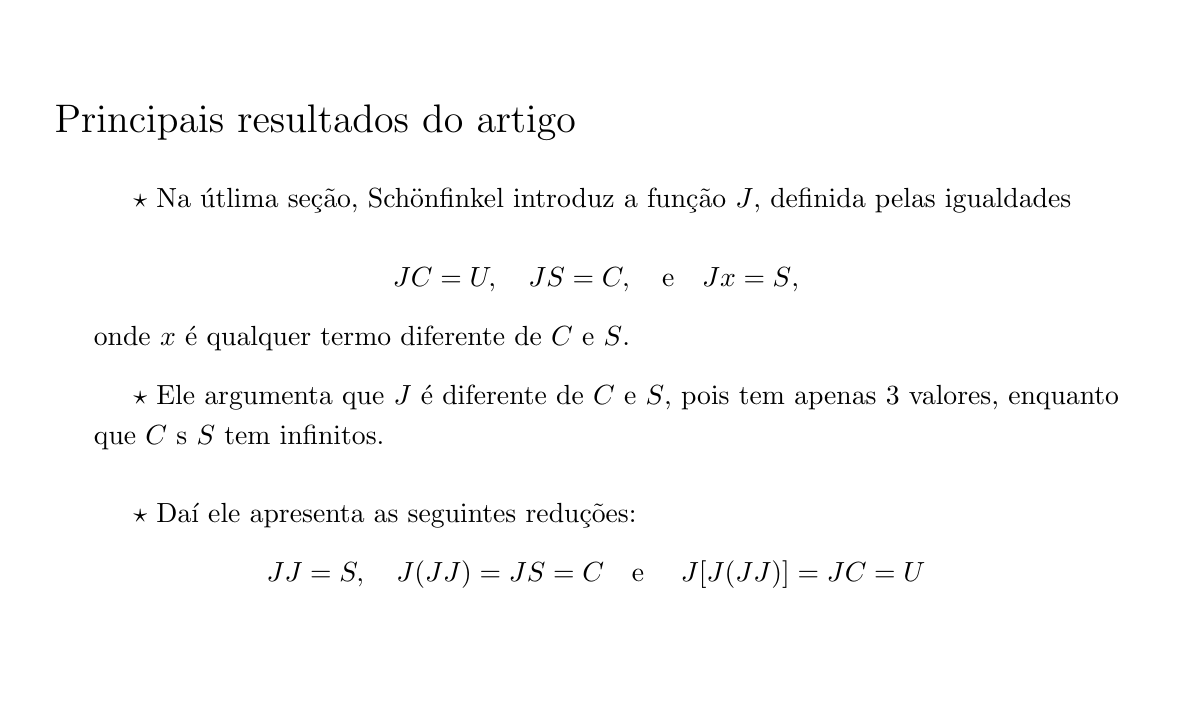
\begin{tikzpicture}
\node[draw,opacity=0] at (0, 0) {x};
\node[draw,opacity=0] at (14, 8) {x};

	\node[anchor=west] (title) at (0.0, 7.0) { \Large \bbbold{Principais resultados do artigo} };


	\node[anchor=west] (a) at (1.0, 6.0) { $\star$ \bbtext{Na útlima seção, Schönfinkel introduz a função $J$, definida pelas igualdades} };

	\node[] (a1) at (7.0, 5.0) { $JC = U,\ \ \ JS = C, \ \ \ \mbox{e}\ \ \ Jx = S$, };

	\node[anchor=west] (a2) at (0.5, 4.25) { \bbtext{onde $x$ é qualquer termo diferente de $C$ e $S$.} };


	\node[anchor=west] (b) at (1.0, 3.5) { $\star$ \bbtext{Ele argumenta que $J$ é diferente de $C$ e $S$, pois tem apenas 3 valores, enquanto} };

	\node[anchor=west] (b1) at (0.5, 3.0) { \bbtext{que $C$ s $S$ tem infinitos.} };


	\node[anchor=west] (c) at (1.0, 2.0) { $\star$ \bbtext{Daí ele apresenta as seguintes reduções: } };

	\node[] (c1) at (7.0, 1.25) { $JJ = S,\ \ \ J(JJ) = JS = C\ \ \ \mbox{e}\ \ \ \ J[J(JJ)] = JC = U$ };

\end{tikzpicture}
\end{frame}
\begin{frame}[plain,t]
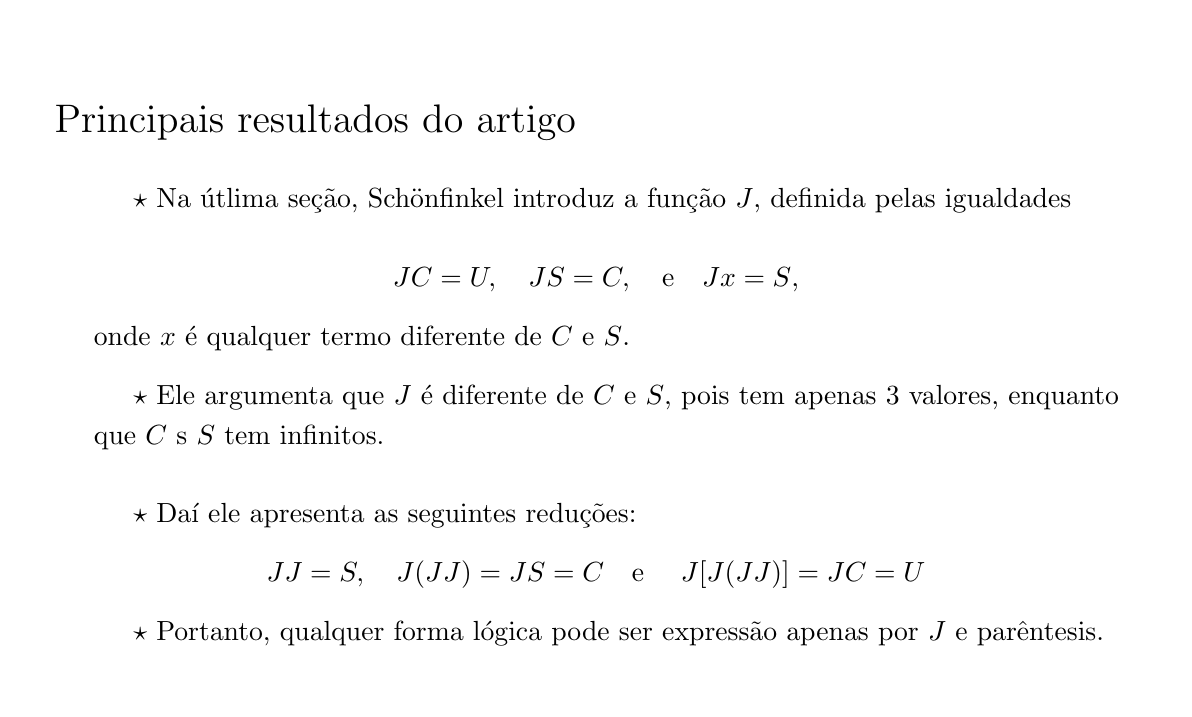
\begin{tikzpicture}
\node[draw,opacity=0] at (0, 0) {x};
\node[draw,opacity=0] at (14, 8) {x};

	\node[anchor=west] (title) at (0.0, 7.0) { \Large \bbbold{Principais resultados do artigo} };


	\node[anchor=west] (a) at (1.0, 6.0) { $\star$ \bbtext{Na útlima seção, Schönfinkel introduz a função $J$, definida pelas igualdades} };

	\node[] (a1) at (7.0, 5.0) { $JC = U,\ \ \ JS = C, \ \ \ \mbox{e}\ \ \ Jx = S$, };

	\node[anchor=west] (a2) at (0.5, 4.25) { \bbtext{onde $x$ é qualquer termo diferente de $C$ e $S$.} };


	\node[anchor=west] (b) at (1.0, 3.5) { $\star$ \bbtext{Ele argumenta que $J$ é diferente de $C$ e $S$, pois tem apenas 3 valores, enquanto} };

	\node[anchor=west] (b1) at (0.5, 3.0) { \bbtext{que $C$ s $S$ tem infinitos.} };


	\node[anchor=west] (c) at (1.0, 2.0) { $\star$ \bbtext{Daí ele apresenta as seguintes reduções: } };

	\node[] (c1) at (7.0, 1.25) { $JJ = S,\ \ \ J(JJ) = JS = C\ \ \ \mbox{e}\ \ \ \ J[J(JJ)] = JC = U$ };


	\node[anchor=west] (d) at (1.0, 0.5) { $\star$ \bbtext{Portanto, qualquer forma lógica pode ser expressão apenas por $J$ e parêntesis.} };

\end{tikzpicture}
\end{frame}
\begin{frame}[plain,t]
\vspace*{\fill}

\begin{tikzpicture}
\node[draw,opacity=0] at (0, 0) {x};
\node[draw,opacity=0] at (14, 8) {x};
\node[anchor=west] (title) at (0.0, 7.0) { \Large \bbbold{Combinadores} };

\node[anchor=west] at (0, 4.5) {\begin{tcolorbox}[colback=blue!5,colframe=blue!60!green,title=\textbf{Definição de combinador}]
\bbtext{Sejam $x_1, x_2, x_3, \ldots, x_N$ termos sem quaisquer restrições. Um combinador $\mathcal{C}$ é uma função destas variáveis
tal que seu valor depende única e exclusivamente de aplicação destes termos e de combinadores previamente definidos.}
\end{tcolorbox}};

\end{tikzpicture}

\vspace*{\fill}
\end{frame}
\begin{frame}[plain,t]
\begin{tikzpicture}
\node[draw,opacity=0] at (0, 0) {x};
\node[draw,opacity=0] at (14, 8) {x};

	\node[anchor=west] (title) at (0.0, 7.0) { \Large \bbbold{Cálculo $SK$} };

\end{tikzpicture}
\end{frame}
\begin{frame}[plain,t]
\begin{tikzpicture}
\node[draw,opacity=0] at (0, 0) {x};
\node[draw,opacity=0] at (14, 8) {x};

	\node[anchor=west] (title) at (0.0, 7.0) { \Large \bbbold{Cálculo $SK$} };


	\node[anchor=west] (a) at (1.0, 6.0) { $\star$ \bbtext{É um sistema computacional minimalista} };

\end{tikzpicture}
\end{frame}
\begin{frame}[plain,t]
\begin{tikzpicture}
\node[draw,opacity=0] at (0, 0) {x};
\node[draw,opacity=0] at (14, 8) {x};

	\node[anchor=west] (title) at (0.0, 7.0) { \Large \bbbold{Cálculo $SK$} };


	\node[anchor=west] (a) at (1.0, 6.0) { $\star$ \bbtext{É um sistema computacional minimalista} };

	\node[anchor=west] (b) at (1.0, 5.0) { $\star$ \bbtext{Todos os objetos são funções unárias} };

\end{tikzpicture}
\end{frame}
\begin{frame}[plain,t]
\begin{tikzpicture}
\node[draw,opacity=0] at (0, 0) {x};
\node[draw,opacity=0] at (14, 8) {x};

	\node[anchor=west] (title) at (0.0, 7.0) { \Large \bbbold{Cálculo $SK$} };


	\node[anchor=west] (a) at (1.0, 6.0) { $\star$ \bbtext{É um sistema computacional minimalista} };

	\node[anchor=west] (b) at (1.0, 5.0) { $\star$ \bbtext{Todos os objetos são funções unárias} };

	\node[anchor=west] (c) at (1.0, 4.0) { $\star$ \bbtext{Há apenas duas primitivas: $S$ e $K$} };

\end{tikzpicture}
\end{frame}
\begin{frame}[plain,t]
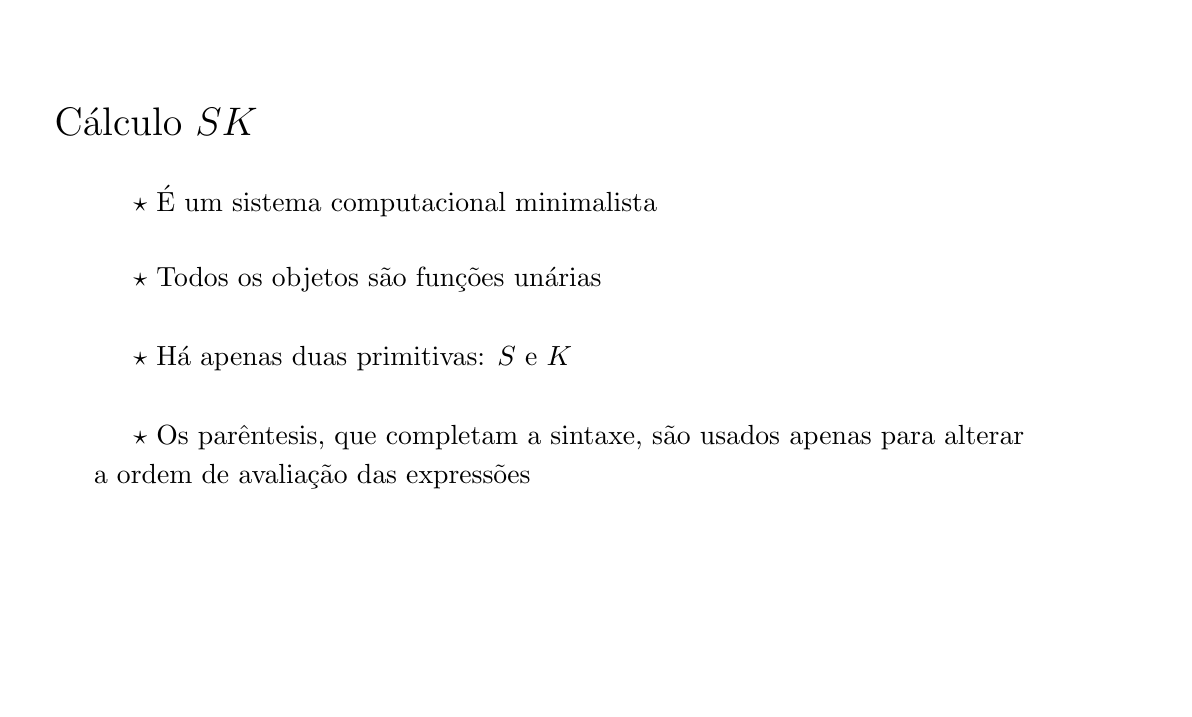
\begin{tikzpicture}
\node[draw,opacity=0] at (0, 0) {x};
\node[draw,opacity=0] at (14, 8) {x};

	\node[anchor=west] (title) at (0.0, 7.0) { \Large \bbbold{Cálculo $SK$} };


	\node[anchor=west] (a) at (1.0, 6.0) { $\star$ \bbtext{É um sistema computacional minimalista} };

	\node[anchor=west] (b) at (1.0, 5.0) { $\star$ \bbtext{Todos os objetos são funções unárias} };

	\node[anchor=west] (c) at (1.0, 4.0) { $\star$ \bbtext{Há apenas duas primitivas: $S$ e $K$} };

	\node[anchor=west] (d) at (1.0, 3.0) { $\star$ \bbtext{Os parêntesis, que completam a sintaxe, são usados apenas para alterar} };

	\node[anchor=west] (d1) at (0.5, 2.5) { \bbtext{a ordem de avaliação das expressões} };

\end{tikzpicture}
\end{frame}
\begin{frame}[plain,t]
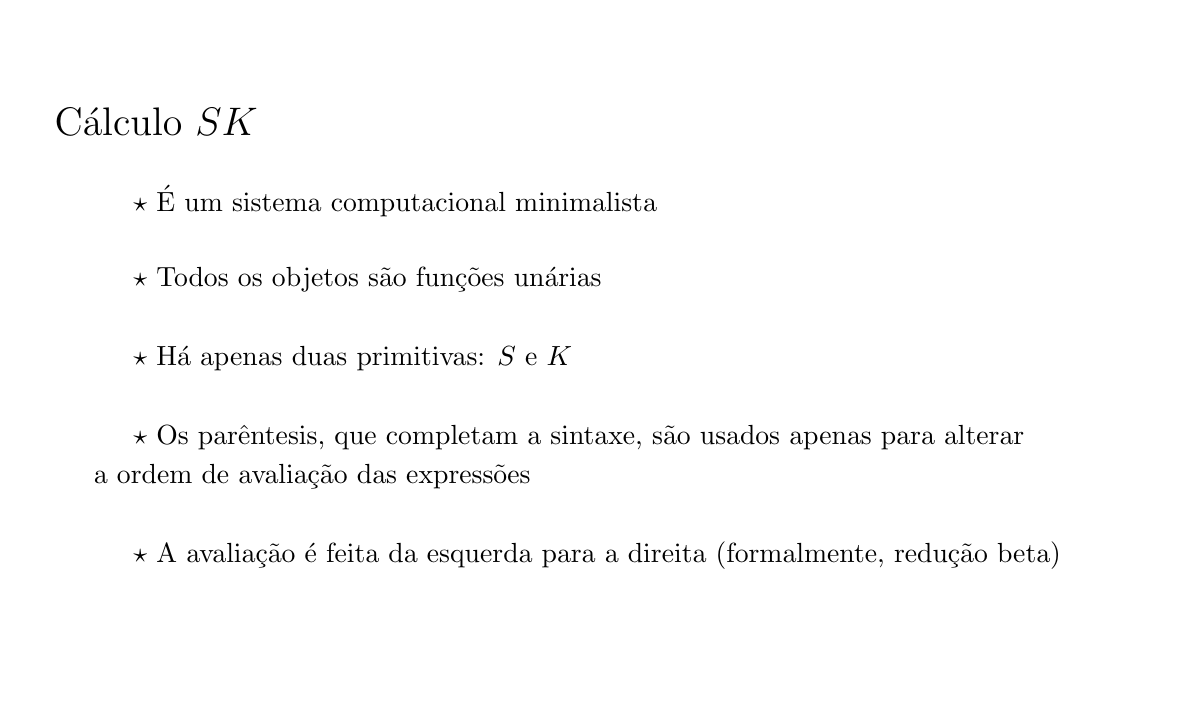
\begin{tikzpicture}
\node[draw,opacity=0] at (0, 0) {x};
\node[draw,opacity=0] at (14, 8) {x};

	\node[anchor=west] (title) at (0.0, 7.0) { \Large \bbbold{Cálculo $SK$} };


	\node[anchor=west] (a) at (1.0, 6.0) { $\star$ \bbtext{É um sistema computacional minimalista} };

	\node[anchor=west] (b) at (1.0, 5.0) { $\star$ \bbtext{Todos os objetos são funções unárias} };

	\node[anchor=west] (c) at (1.0, 4.0) { $\star$ \bbtext{Há apenas duas primitivas: $S$ e $K$} };

	\node[anchor=west] (d) at (1.0, 3.0) { $\star$ \bbtext{Os parêntesis, que completam a sintaxe, são usados apenas para alterar} };

	\node[anchor=west] (d1) at (0.5, 2.5) { \bbtext{a ordem de avaliação das expressões} };

	\node[anchor=west] (e) at (1.0, 1.5) { $\star$ \bbtext{A avaliação é feita da esquerda para a direita (formalmente, redução beta)} };

\end{tikzpicture}
\end{frame}
\begin{frame}[plain,t]
\begin{tikzpicture}
\node[draw,opacity=0] at (0, 0) {x};
\node[draw,opacity=0] at (14, 8) {x};

	\node[anchor=west] (title) at (0.0, 7.0) { \Large \bbbold{Redução beta} };

\end{tikzpicture}
\end{frame}
\begin{frame}[plain,t]
\begin{tikzpicture}
\node[draw,opacity=0] at (0, 0) {x};
\node[draw,opacity=0] at (14, 8) {x};

	\node[anchor=west] (title) at (0.0, 7.0) { \Large \bbbold{Redução beta} };

	\node[anchor=west] (a) at (0.5, 6.0) { $\star$ \bbtext{Inicia aplicando a subexpressão mais à esquerda, se houverem argumentos suficiente} };

\end{tikzpicture}
\end{frame}
\begin{frame}[plain,t]
\begin{tikzpicture}
\node[draw,opacity=0] at (0, 0) {x};
\node[draw,opacity=0] at (14, 8) {x};

	\node[anchor=west] (title) at (0.0, 7.0) { \Large \bbbold{Redução beta} };

	\node[anchor=west] (a) at (0.5, 6.0) { $\star$ \bbtext{Inicia aplicando a subexpressão mais à esquerda, se houverem argumentos suficiente} };

	\node[anchor=west] (b) at (0.5, 5.0) { $\star$ \bbtext{Subexpressões à direita não são avaliadas (\bbenglish{lazy evaluation})} };

\end{tikzpicture}
\end{frame}
\begin{frame}[plain,t]
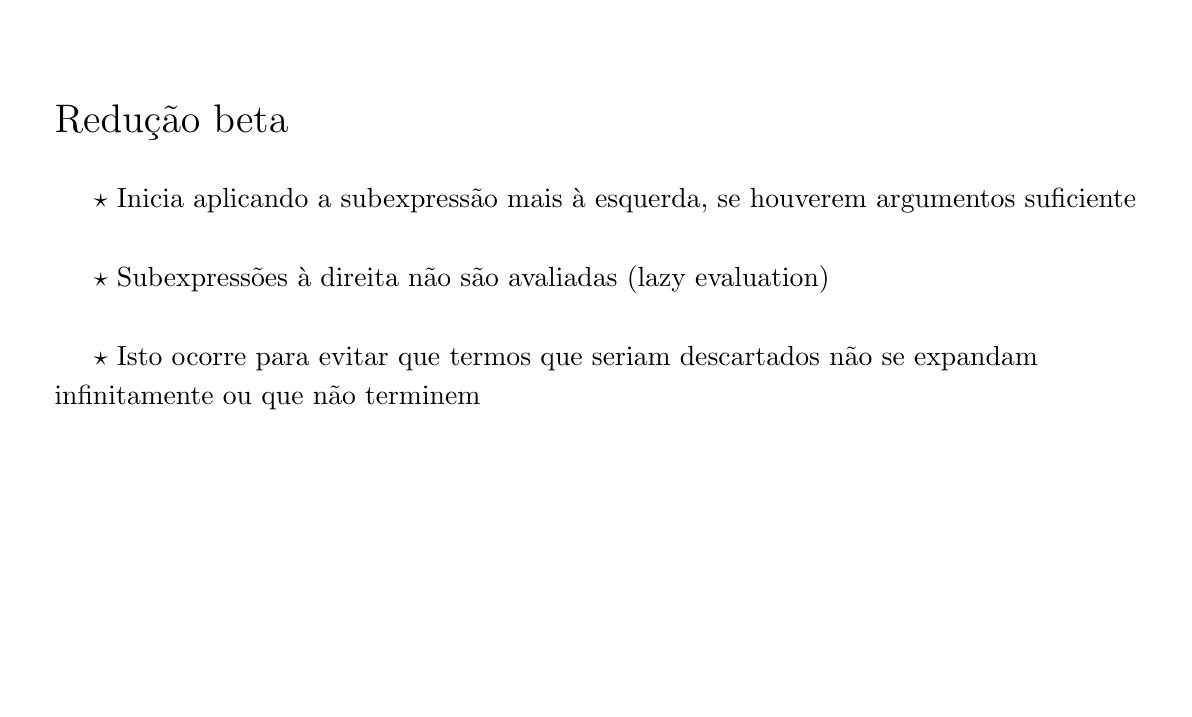
\begin{tikzpicture}
\node[draw,opacity=0] at (0, 0) {x};
\node[draw,opacity=0] at (14, 8) {x};

	\node[anchor=west] (title) at (0.0, 7.0) { \Large \bbbold{Redução beta} };

	\node[anchor=west] (a) at (0.5, 6.0) { $\star$ \bbtext{Inicia aplicando a subexpressão mais à esquerda, se houverem argumentos suficiente} };

	\node[anchor=west] (b) at (0.5, 5.0) { $\star$ \bbtext{Subexpressões à direita não são avaliadas (\bbenglish{lazy evaluation})} };

	\node[anchor=west] (c) at (0.5, 4.0) { $\star$ \bbtext{Isto ocorre para evitar que termos que seriam descartados não se expandam } };

	\node[anchor=west] (c1) at (0.0, 3.5) { \bbtext{infinitamente ou que não terminem} };


\end{tikzpicture}
\end{frame}
\begin{frame}[plain,t]
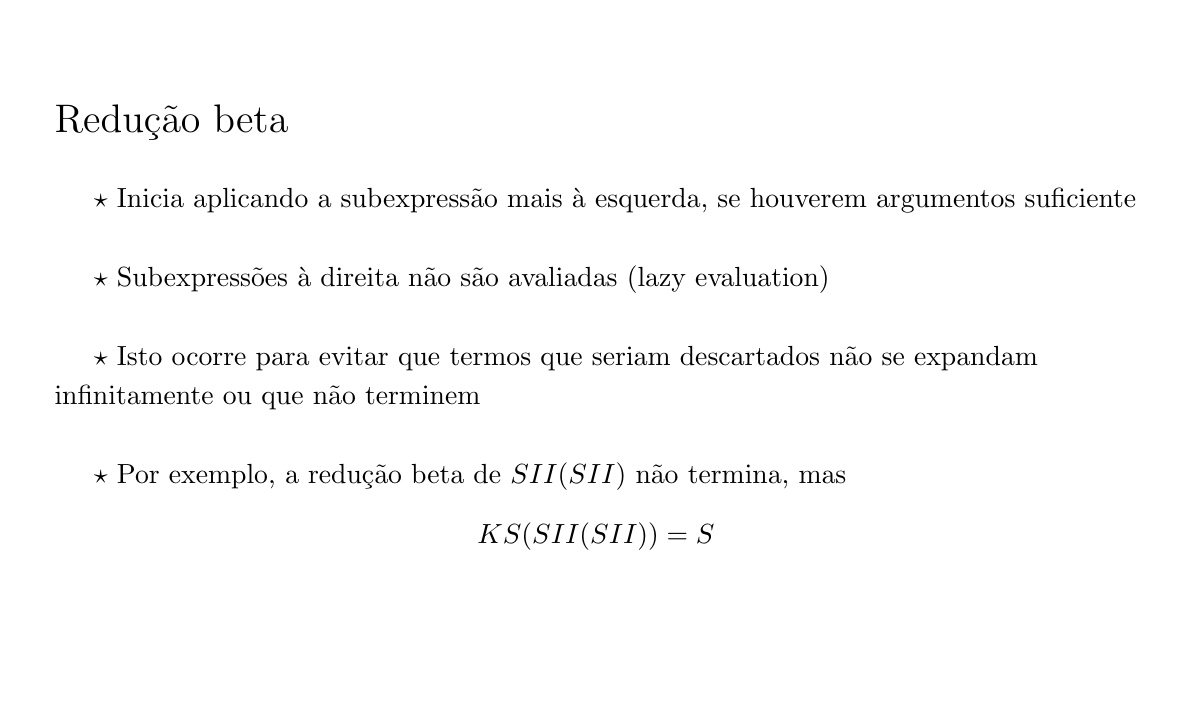
\begin{tikzpicture}
\node[draw,opacity=0] at (0, 0) {x};
\node[draw,opacity=0] at (14, 8) {x};

	\node[anchor=west] (title) at (0.0, 7.0) { \Large \bbbold{Redução beta} };

	\node[anchor=west] (a) at (0.5, 6.0) { $\star$ \bbtext{Inicia aplicando a subexpressão mais à esquerda, se houverem argumentos suficiente} };

	\node[anchor=west] (b) at (0.5, 5.0) { $\star$ \bbtext{Subexpressões à direita não são avaliadas (\bbenglish{lazy evaluation})} };

	\node[anchor=west] (c) at (0.5, 4.0) { $\star$ \bbtext{Isto ocorre para evitar que termos que seriam descartados não se expandam } };

	\node[anchor=west] (c1) at (0.0, 3.5) { \bbtext{infinitamente ou que não terminem} };


	\node[anchor=west] (d) at (0.5, 2.5) { $\star$ \bbtext{Por exemplo, a redução beta de $SII(SII)$ não termina, mas} };

	\node[] (d1) at (7.0, 1.74) { $KS(SII(SII)) = S$ };

\end{tikzpicture}
\end{frame}
\begin{frame}[plain,t]
\begin{tikzpicture}
\node[draw,opacity=0] at (0, 0) {x};
\node[draw,opacity=0] at (14, 8) {x};

	\node[anchor=west] (title) at (0.0, 7.0) { \Large \bbbold{Combinador $M$} };

\end{tikzpicture}
\end{frame}
\begin{frame}[plain,t]
\begin{tikzpicture}
\node[draw,opacity=0] at (0, 0) {x};
\node[draw,opacity=0] at (14, 8) {x};

	\node[anchor=west] (title) at (0.0, 7.0) { \Large \bbbold{Combinador $M$} };

	\node[] (mockingbird) at (11.0, 4.5) { \includegraphics[scale=0.035]{figs/mockingbird.jpg} };

	\node[] (label) at (11.0, 2.0) { \footnotesize \bbtext{Tordo-imitador (\bbenglish{mockingbird})} };

\end{tikzpicture}
\end{frame}
\begin{frame}[plain,t]
\begin{tikzpicture}
\node[draw,opacity=0] at (0, 0) {x};
\node[draw,opacity=0] at (14, 8) {x};

	\node[anchor=west] (title) at (0.0, 7.0) { \Large \bbbold{Combinador $M$} };

	\node[] (mockingbird) at (11.0, 4.5) { \includegraphics[scale=0.035]{figs/mockingbird.jpg} };

	\node[] (label) at (11.0, 2.0) { \footnotesize \bbtext{Tordo-imitador (\bbenglish{mockingbird})} };

	\node[anchor=west] (a) at (1.0, 6.0) { $\star$ \bbtext{Por definição, $Mx = xx$} };

\end{tikzpicture}
\end{frame}
\begin{frame}[plain,t]
\begin{tikzpicture}
\node[draw,opacity=0] at (0, 0) {x};
\node[draw,opacity=0] at (14, 8) {x};

	\node[anchor=west] (title) at (0.0, 7.0) { \Large \bbbold{Combinador $M$} };

	\node[] (mockingbird) at (11.0, 4.5) { \includegraphics[scale=0.035]{figs/mockingbird.jpg} };

	\node[] (label) at (11.0, 2.0) { \footnotesize \bbtext{Tordo-imitador (\bbenglish{mockingbird})} };

	\node[anchor=west] (a) at (1.0, 6.0) { $\star$ \bbtext{Por definição, $Mx = xx$} };

	\node[anchor=west] (b) at (1.0, 5.0) { $\star$ \bbtext{Observe que:} };

	\node[anchor=west] (b1) at (2.0, 4.0) { $Ma = aa = Ia(Ia) = SIIa$ };

\end{tikzpicture}
\end{frame}
\begin{frame}[plain,t]
\begin{tikzpicture}
\node[draw,opacity=0] at (0, 0) {x};
\node[draw,opacity=0] at (14, 8) {x};

	\node[anchor=west] (title) at (0.0, 7.0) { \Large \bbbold{Combinador $M$} };

	\node[] (mockingbird) at (11.0, 4.5) { \includegraphics[scale=0.035]{figs/mockingbird.jpg} };

	\node[] (label) at (11.0, 2.0) { \footnotesize \bbtext{Tordo-imitador (\bbenglish{mockingbird})} };

	\node[anchor=west] (a) at (1.0, 6.0) { $\star$ \bbtext{Por definição, $Mx = xx$} };

	\node[anchor=west] (b) at (1.0, 5.0) { $\star$ \bbtext{Observe que:} };

	\node[anchor=west] (b1) at (2.0, 4.0) { $Ma = aa = Ia(Ia) = SIIa$ };

	\node[anchor=west] (c) at (1.0, 3.0) { $\star$ \bbtext{Portanto, $M = SII$} };

\end{tikzpicture}
\end{frame}
\begin{frame}[plain,t]
\begin{tikzpicture}
\node[draw,opacity=0] at (0, 0) {x};
\node[draw,opacity=0] at (14, 8) {x};

	\node[anchor=west] (title) at (0.0, 7.0) { \Large \bbbold{Combinador $M$} };

	\node[] (mockingbird) at (11.0, 4.5) { \includegraphics[scale=0.035]{figs/mockingbird.jpg} };

	\node[] (label) at (11.0, 2.0) { \footnotesize \bbtext{Tordo-imitador (\bbenglish{mockingbird})} };

	\node[anchor=west] (a) at (1.0, 6.0) { $\star$ \bbtext{Por definição, $Mx = xx$} };

	\node[anchor=west] (b) at (1.0, 5.0) { $\star$ \bbtext{Observe que:} };

	\node[anchor=west] (b1) at (2.0, 4.0) { $Ma = aa = Ia(Ia) = SIIa$ };

	\node[anchor=west] (c) at (1.0, 3.0) { $\star$ \bbtext{Portanto, $M = SII$} };

	\node[anchor=west] (d) at (1.0, 2.0) { $\star$ \bbtext{A redução beta de $MM$ não termina} };

\end{tikzpicture}
\end{frame}
\begin{frame}[plain,t]
\begin{tikzpicture}
\node[draw,opacity=0] at (0, 0) {x};
\node[draw,opacity=0] at (14, 8) {x};

	\node[anchor=west] (title) at (0.0, 7.0) { \Large \bbbold{\textit{To Mock a Mockingbird}} };

\end{tikzpicture}
\end{frame}
\begin{frame}[plain,t]
\begin{tikzpicture}
\node[draw,opacity=0] at (0, 0) {x};
\node[draw,opacity=0] at (14, 8) {x};

	\node[anchor=west] (title) at (0.0, 7.0) { \Large \bbbold{\textit{To Mock a Mockingbird}} };

	\node[anchor=west] (a) at (0.5, 6.0) { \bbbold{Definições:} };

\end{tikzpicture}
\end{frame}
\begin{frame}[plain,t]
\begin{tikzpicture}
\node[draw,opacity=0] at (0, 0) {x};
\node[draw,opacity=0] at (14, 8) {x};

	\node[anchor=west] (title) at (0.0, 7.0) { \Large \bbbold{\textit{To Mock a Mockingbird}} };

	\node[anchor=west] (a) at (0.5, 6.0) { \bbbold{Definições:} };

	\node[anchor=west] (b) at (1.0, 5.0) { $\star$ \bbtext{As letras maiúsculas ($A, B, \ldots$) são pássaros} };

\end{tikzpicture}
\end{frame}
\begin{frame}[plain,t]
\begin{tikzpicture}
\node[draw,opacity=0] at (0, 0) {x};
\node[draw,opacity=0] at (14, 8) {x};

	\node[anchor=west] (title) at (0.0, 7.0) { \Large \bbbold{\textit{To Mock a Mockingbird}} };

	\node[anchor=west] (a) at (0.5, 6.0) { \bbbold{Definições:} };

	\node[anchor=west] (b) at (1.0, 5.0) { $\star$ \bbtext{As letras maiúsculas ($A, B, \ldots$) são pássaros} };

	\node[anchor=west] (c) at (1.0, 4.0) { $\star$ \bbtext{Quando o pássaro $A$ ouve o nome do pássaro $B$, ele responde o nome do} };

	\node[anchor=west] (c1) at (0.5, 3.5) { \bbtext{pássaro $AB$} };

\end{tikzpicture}
\end{frame}
\begin{frame}[plain,t]
\begin{tikzpicture}
\node[draw,opacity=0] at (0, 0) {x};
\node[draw,opacity=0] at (14, 8) {x};

	\node[anchor=west] (title) at (0.0, 7.0) { \Large \bbbold{\textit{To Mock a Mockingbird}} };

	\node[anchor=west] (a) at (0.5, 6.0) { \bbbold{Definições:} };

	\node[anchor=west] (b) at (1.0, 5.0) { $\star$ \bbtext{As letras maiúsculas ($A, B, \ldots$) são pássaros} };

	\node[anchor=west] (c) at (1.0, 4.0) { $\star$ \bbtext{Quando o pássaro $A$ ouve o nome do pássaro $B$, ele responde o nome do} };

	\node[anchor=west] (c1) at (0.5, 3.5) { \bbtext{pássaro $AB$} };

	\node[anchor=west] (d) at (1.0, 2.5) { $\star$ \bbtext{Em geral, $AB\neq BA$} };

\end{tikzpicture}
\end{frame}
\begin{frame}[plain,t]
\begin{tikzpicture}
\node[draw,opacity=0] at (0, 0) {x};
\node[draw,opacity=0] at (14, 8) {x};

	\node[anchor=west] (title) at (0.0, 7.0) { \Large \bbbold{\textit{To Mock a Mockingbird}} };

	\node[anchor=west] (a) at (0.5, 6.0) { \bbbold{Definições:} };

	\node[anchor=west] (b) at (1.0, 5.0) { $\star$ \bbtext{As letras maiúsculas ($A, B, \ldots$) são pássaros} };

	\node[anchor=west] (c) at (1.0, 4.0) { $\star$ \bbtext{Quando o pássaro $A$ ouve o nome do pássaro $B$, ele responde o nome do} };

	\node[anchor=west] (c1) at (0.5, 3.5) { \bbtext{pássaro $AB$} };

	\node[anchor=west] (d) at (1.0, 2.5) { $\star$ \bbtext{Em geral, $AB\neq BA$} };

	\node[anchor=west] (e) at (1.0, 1.5) { $\star$ \bbtext{Para três pássaros quaisquer $A, B, C$, temos que $(AB)C$ e $A(BC)$ não são,} };

	\node[anchor=west] (e1) at (0.5, 1.0) { \bbtext{necessariamente, iguais} };

\end{tikzpicture}
\end{frame}
\begin{frame}[plain,t]
\begin{tikzpicture}
\node[draw,opacity=0] at (0, 0) {x};
\node[draw,opacity=0] at (14, 8) {x};

	\node[anchor=west] (title) at (0.0, 7.0) { \Large \bbbold{\textit{The Significance of the Mockinbird}} };

\end{tikzpicture}
\end{frame}
\begin{frame}[plain,t]
\begin{tikzpicture}
\node[draw,opacity=0] at (0, 0) {x};
\node[draw,opacity=0] at (14, 8) {x};

	\node[anchor=west] (title) at (0.0, 7.0) { \Large \bbbold{\textit{The Significance of the Mockinbird}} };

	\node[anchor=west] (a) at (1.0, 6.0) { $\star$ \bbtext{Se, ao ouvir o nome do pássaro $B$, $A$ responde $B$, dizemos que $A$ gosta de $B$} };

\end{tikzpicture}
\end{frame}
\begin{frame}[plain,t]
\begin{tikzpicture}
\node[draw,opacity=0] at (0, 0) {x};
\node[draw,opacity=0] at (14, 8) {x};

	\node[anchor=west] (title) at (0.0, 7.0) { \Large \bbbold{\textit{The Significance of the Mockinbird}} };

	\node[anchor=west] (a) at (1.0, 6.0) { $\star$ \bbtext{Se, ao ouvir o nome do pássaro $B$, $A$ responde $B$, dizemos que $A$ gosta de $B$} };

	\node[anchor=west] (b) at (1.0, 5.0) { $\star$ \bbtext{Em notação simbólica, $A$ gosta de $B$ se $AB = B$} };

\end{tikzpicture}
\end{frame}
\begin{frame}[plain,t]
\begin{tikzpicture}
\node[draw,opacity=0] at (0, 0) {x};
\node[draw,opacity=0] at (14, 8) {x};

	\node[anchor=west] (title) at (0.0, 7.0) { \Large \bbbold{\textit{The Significance of the Mockinbird}} };

	\node[anchor=west] (a) at (1.0, 6.0) { $\star$ \bbtext{Se, ao ouvir o nome do pássaro $B$, $A$ responde $B$, dizemos que $A$ gosta de $B$} };

	\node[anchor=west] (b) at (1.0, 5.0) { $\star$ \bbtext{Em notação simbólica, $A$ gosta de $B$ se $AB = B$} };

	\node[anchor=west] (c) at (1.0, 4.0) { $\star$ \bbtext{Assuma que, na floresta, para quaisquer dois pássaros $A$ e $B$ existe um pássaro $C$} };

	\node[anchor=west] (c1) at (0.5, 3.5) { \bbtext{tal que, para qualquer pássaro $x$, $Cx = A(Bx)$} };

\end{tikzpicture}
\end{frame}
\begin{frame}[plain,t]
\begin{tikzpicture}
\node[draw,opacity=0] at (0, 0) {x};
\node[draw,opacity=0] at (14, 8) {x};

	\node[anchor=west] (title) at (0.0, 7.0) { \Large \bbbold{\textit{The Significance of the Mockinbird}} };

	\node[anchor=west] (a) at (1.0, 6.0) { $\star$ \bbtext{Se, ao ouvir o nome do pássaro $B$, $A$ responde $B$, dizemos que $A$ gosta de $B$} };

	\node[anchor=west] (b) at (1.0, 5.0) { $\star$ \bbtext{Em notação simbólica, $A$ gosta de $B$ se $AB = B$} };

	\node[anchor=west] (c) at (1.0, 4.0) { $\star$ \bbtext{Assuma que, na floresta, para quaisquer dois pássaros $A$ e $B$ existe um pássaro $C$} };

	\node[anchor=west] (c1) at (0.5, 3.5) { \bbtext{tal que, para qualquer pássaro $x$, $Cx = A(Bx)$} };

	\node[anchor=west] (d) at (1.0, 2.5) { $\star$ \bbtext{Assuma também que o tordo-imitador $M$ mora na floresta} };

\end{tikzpicture}
\end{frame}
\begin{frame}[plain,t]
\begin{tikzpicture}
\node[draw,opacity=0] at (0, 0) {x};
\node[draw,opacity=0] at (14, 8) {x};

	\node[anchor=west] (title) at (0.0, 7.0) { \Large \bbbold{\textit{The Significance of the Mockinbird}} };

	\node[anchor=west] (a) at (1.0, 6.0) { $\star$ \bbtext{Se, ao ouvir o nome do pássaro $B$, $A$ responde $B$, dizemos que $A$ gosta de $B$} };

	\node[anchor=west] (b) at (1.0, 5.0) { $\star$ \bbtext{Em notação simbólica, $A$ gosta de $B$ se $AB = B$} };

	\node[anchor=west] (c) at (1.0, 4.0) { $\star$ \bbtext{Assuma que, na floresta, para quaisquer dois pássaros $A$ e $B$ existe um pássaro $C$} };

	\node[anchor=west] (c1) at (0.5, 3.5) { \bbtext{tal que, para qualquer pássaro $x$, $Cx = A(Bx)$} };

	\node[anchor=west] (d) at (1.0, 2.5) { $\star$ \bbtext{Assuma também que o tordo-imitador $M$ mora na floresta} };

	\node[anchor=west] (e) at (1.0, 1.5) { $\star$ \bbtext{Há dois rumores na floresta: $(a)$ que todo pássaro da floresta gosta de alguém; e } };

	\node[anchor=west] (e1) at (0.5, 1.0) { \bbtext{$(b)$ que existe ao menos um pássaro que não gosta de ninguém} };

\end{tikzpicture}
\end{frame}
\begin{frame}[plain,t]
\begin{tikzpicture}
\node[draw,opacity=0] at (0, 0) {x};
\node[draw,opacity=0] at (14, 8) {x};

	\node[anchor=west] (title) at (0.0, 7.0) { \Large \bbbold{\textit{The Significance of the Mockinbird}} };

	\node[anchor=west] (a) at (1.0, 6.0) { $\star$ \bbtext{Se, ao ouvir o nome do pássaro $B$, $A$ responde $B$, dizemos que $A$ gosta de $B$} };

	\node[anchor=west] (b) at (1.0, 5.0) { $\star$ \bbtext{Em notação simbólica, $A$ gosta de $B$ se $AB = B$} };

	\node[anchor=west] (c) at (1.0, 4.0) { $\star$ \bbtext{Assuma que, na floresta, para quaisquer dois pássaros $A$ e $B$ existe um pássaro $C$} };

	\node[anchor=west] (c1) at (0.5, 3.5) { \bbtext{tal que, para qualquer pássaro $x$, $Cx = A(Bx)$} };

	\node[anchor=west] (d) at (1.0, 2.5) { $\star$ \bbtext{Assuma também que o tordo-imitador $M$ mora na floresta} };

	\node[anchor=west] (e) at (1.0, 1.5) { $\star$ \bbtext{Há dois rumores na floresta: $(a)$ que todo pássaro da floresta gosta de alguém; e } };

	\node[anchor=west] (e1) at (0.5, 1.0) { \bbtext{$(b)$ que existe ao menos um pássaro que não gosta de ninguém} };

	\node[anchor=west] (g) at (1.0, 0.0) { $\star$ \bbtext{Qual dos dois rumores é verdadeiro?} };

\end{tikzpicture}
\end{frame}
\begin{frame}[plain,t]
\begin{tikzpicture}
\node[draw,opacity=0] at (0, 0) {x};
\node[draw,opacity=0] at (14, 8) {x};

	\node[anchor=west] (title) at (0.0, 7.0) { \Large \bbbold{Solução} };

\end{tikzpicture}
\end{frame}
\begin{frame}[plain,t]
\begin{tikzpicture}
\node[draw,opacity=0] at (0, 0) {x};
\node[draw,opacity=0] at (14, 8) {x};

	\node[anchor=west] (title) at (0.0, 7.0) { \Large \bbbold{Solução} };

	\node[anchor=west] (a) at (1.0, 6.0) { $\star$ \bbtext{Seja $C$ o pássaro que compõem $A$ e $M$, isto é, $Cx = A(Mx)$ para qualquer} };

	\node[anchor=west] (a1) at (0.5, 5.5) { \bbtext{pássaro $x$} };

\end{tikzpicture}
\end{frame}
\begin{frame}[plain,t]
\begin{tikzpicture}
\node[draw,opacity=0] at (0, 0) {x};
\node[draw,opacity=0] at (14, 8) {x};

	\node[anchor=west] (title) at (0.0, 7.0) { \Large \bbbold{Solução} };

	\node[anchor=west] (a) at (1.0, 6.0) { $\star$ \bbtext{Seja $C$ o pássaro que compõem $A$ e $M$, isto é, $Cx = A(Mx)$ para qualquer} };

	\node[anchor=west] (a1) at (0.5, 5.5) { \bbtext{pássaro $x$} };

	\node[anchor=west] (b) at (1.0, 4.5) { $\star$ \bbtext{Quando $C$ escuta seu próprio nome, qual é o pássaro que ele responde?} };

\end{tikzpicture}
\end{frame}
\begin{frame}[plain,t]
\begin{tikzpicture}
\node[draw,opacity=0] at (0, 0) {x};
\node[draw,opacity=0] at (14, 8) {x};

	\node[anchor=west] (title) at (0.0, 7.0) { \Large \bbbold{Solução} };

	\node[anchor=west] (a) at (1.0, 6.0) { $\star$ \bbtext{Seja $C$ o pássaro que compõem $A$ e $M$, isto é, $Cx = A(Mx)$ para qualquer} };

	\node[anchor=west] (a1) at (0.5, 5.5) { \bbtext{pássaro $x$} };

	\node[anchor=west] (b) at (1.0, 4.5) { $\star$ \bbtext{Quando $C$ escuta seu próprio nome, qual é o pássaro que ele responde?} };

	\node[anchor=west] (c) at (1.0, 3.5) { $\star$ \bbtext{Temos que $CC = A(MC)$, o que equivale a $A(MC) = CC$} };

\end{tikzpicture}
\end{frame}
\begin{frame}[plain,t]
\begin{tikzpicture}
\node[draw,opacity=0] at (0, 0) {x};
\node[draw,opacity=0] at (14, 8) {x};

	\node[anchor=west] (title) at (0.0, 7.0) { \Large \bbbold{Solução} };

	\node[anchor=west] (a) at (1.0, 6.0) { $\star$ \bbtext{Seja $C$ o pássaro que compõem $A$ e $M$, isto é, $Cx = A(Mx)$ para qualquer} };

	\node[anchor=west] (a1) at (0.5, 5.5) { \bbtext{pássaro $x$} };

	\node[anchor=west] (b) at (1.0, 4.5) { $\star$ \bbtext{Quando $C$ escuta seu próprio nome, qual é o pássaro que ele responde?} };

	\node[anchor=west] (c) at (1.0, 3.5) { $\star$ \bbtext{Temos que $CC = A(MC)$, o que equivale a $A(MC) = CC$} };

	\node[anchor=west] (d) at (1.0, 2.5) { $\star$ \bbtext{Quando ouve $C$, o tordo-imitador responde $MC = CC$} };

\end{tikzpicture}
\end{frame}
\begin{frame}[plain,t]
\begin{tikzpicture}
\node[draw,opacity=0] at (0, 0) {x};
\node[draw,opacity=0] at (14, 8) {x};

	\node[anchor=west] (title) at (0.0, 7.0) { \Large \bbbold{Solução} };

	\node[anchor=west] (a) at (1.0, 6.0) { $\star$ \bbtext{Seja $C$ o pássaro que compõem $A$ e $M$, isto é, $Cx = A(Mx)$ para qualquer} };

	\node[anchor=west] (a1) at (0.5, 5.5) { \bbtext{pássaro $x$} };

	\node[anchor=west] (b) at (1.0, 4.5) { $\star$ \bbtext{Quando $C$ escuta seu próprio nome, qual é o pássaro que ele responde?} };

	\node[anchor=west] (c) at (1.0, 3.5) { $\star$ \bbtext{Temos que $CC = A(MC)$, o que equivale a $A(MC) = CC$} };

	\node[anchor=west] (d) at (1.0, 2.5) { $\star$ \bbtext{Quando ouve $C$, o tordo-imitador responde $MC = CC$} };

	\node[anchor=west] (e) at (1.0, 1.5) { $\star$ \bbtext{Assim, quando ouve o nome do pássaro $MC$, o pássaro $A$ responde} };

	\node[] (e1) at (7.0, 0.75) { $A(MC) = CC = MC$ };

\end{tikzpicture}
\end{frame}
\begin{frame}[plain,t]
\begin{tikzpicture}
\node[draw,opacity=0] at (0, 0) {x};
\node[draw,opacity=0] at (14, 8) {x};

	\node[anchor=west] (title) at (0.0, 7.0) { \Large \bbbold{Solução} };

	\node[anchor=west] (a) at (1.0, 6.0) { $\star$ \bbtext{Seja $C$ o pássaro que compõem $A$ e $M$, isto é, $Cx = A(Mx)$ para qualquer} };

	\node[anchor=west] (a1) at (0.5, 5.5) { \bbtext{pássaro $x$} };

	\node[anchor=west] (b) at (1.0, 4.5) { $\star$ \bbtext{Quando $C$ escuta seu próprio nome, qual é o pássaro que ele responde?} };

	\node[anchor=west] (c) at (1.0, 3.5) { $\star$ \bbtext{Temos que $CC = A(MC)$, o que equivale a $A(MC) = CC$} };

	\node[anchor=west] (d) at (1.0, 2.5) { $\star$ \bbtext{Quando ouve $C$, o tordo-imitador responde $MC = CC$} };

	\node[anchor=west] (e) at (1.0, 1.5) { $\star$ \bbtext{Assim, quando ouve o nome do pássaro $MC$, o pássaro $A$ responde} };

	\node[] (e1) at (7.0, 0.75) { $A(MC) = CC = MC$ };

	\node[anchor=west] (f) at (1.0, 0.0) { $\star$ \bbtext{Portanto, o primeiro rumor é o verdadeiro} };

\end{tikzpicture}
\end{frame}
\begin{frame}[plain,t]
\begin{tikzpicture}
\node[draw,opacity=0] at (0, 0) {x};
\node[draw,opacity=0] at (14, 8) {x};

	\node[anchor=west] (title) at (0.0, 6.5) { \Large \bbbold{Referências} };

	\node[anchor=west] (a) at (1.0, 5.0) { $\star$ \bbbold{USDA.} \href{https://www.aphis.usda.gov/operational-wildlife-activities/starlings-blackbirds}{\bbenglish{Operational Activities: Starlings and Blackbirds}}\bbtext{. Acesso em 07/04/2025.} };

	\node[anchor=west] (b) at (1.0, 4.0) { $\star$ \bbbold{CornellLab.} \href{https://www.allaboutbirds.org/guide/American_Kestrel/id}{\bbenglish{American Kestrel: Identification}}\bbtext{. Acesso em 07/04/2025.} };

	\node[anchor=west] (c) at (1.0, 3.0) { $\star$ \bbbold{HAYASHI}\bbtext{, Tobias.} \href{https://www.tobiashayashi.com/blog/2019/1/23/the-rare-idiot-bird}{\bbenglish{The rare `idiot bird'}}\bbtext{. Acesso em 07/04/2025}. };

	\node[anchor=west] (d) at (1.0, 2.0) { $\star$ \bbbold{Wikipédia.} \href{https://en.wikipedia.org/wiki/Bluebird}{\bbenglish{Bluebird}}\bbtext{. Acesso em 07/04/2025.} };

	\node[anchor=west] (e) at (1.0, 1.0) { $\star$ \bbbold{Tucson Bird Alliance.} \href{https://tucsonbirds.org/bird_profile/northern-cardinal/?ref=tas}{\bbenglish{Northern Cardinal}}\bbtext{. Acesso em 08/04/2025.} };

\end{tikzpicture}
\end{frame}
\begin{frame}[plain,t]
\begin{tikzpicture}
\node[draw,opacity=0] at (0, 0) {x};
\node[draw,opacity=0] at (14, 8) {x};

	\node[anchor=west] (title) at (0.0, 6.5) { \Large \bbbold{Referências} };

	\node[anchor=west] (a) at (1.0, 5.0) { $\star$ \bbbold{Wikipédia.} \href{https://en.wikipedia.org/wiki/Combinatory_logic}{\bbenglish{Combinatory Logic}}\bbtext{. Acesso em 08/04/2025.} };

	\node[anchor=west] (b) at (1.0, 4.0) { $\star$ \bbbold{AMIKO}\bbtext{, Komi.} \href{https://komiamiko.me/math/ordinals/2020/06/21/ski-numerals.html}{\bbenglish{Large Numbers in the SKI combinador calculus}}\bbtext{. Acesso em 10/04/2025.} };

	\node[anchor=west] (c) at (1.0, 3.0) { $\star$ \bbbold{CornellLab.} \href{https://www.allaboutbirds.org/guide/Northern_Mockingbird/id}{\bbenglish{Northern Mockingbird}}\bbtext{. Acesso em 11/04/2025.} };

	\node[anchor=west] (d) at (1.0, 2.0) { $\star$ \bbbold{SMULLYAN}\bbtext{, Raymond M.} \href{https://www.amazon.com.br/Mock-Mockingbird-Other-Logic-Puzzles/dp/0192801422}{\bbenglish{To Mock a Mockingbird and Other Logic Puzzles}}\bbtext{. Oxford} };

	\node[anchor=west] (d1) at (0.5, 1.5) { \bbtext{Press, 2000.} };


\end{tikzpicture}
\end{frame}
\end{document}
